\newpage
\chapter{Resultados}
\label{chap:resultados}

Este capítulo apresenta os resultados obtidos com a implementação do \textit{pipeline} de detecção de estados operacionais baseado em K-Means para equipamentos industriais elétricos e mecânicos. O sistema processa automaticamente dados de diferentes tipos de equipamentos, utilizando algoritmos de aprendizado não supervisionado para classificação de estados LIGADO/DESLIGADO.

\section{Dados Processados}

O \textit{pipeline} foi executado com dados reais de cinco equipamentos industriais processados em novembro de 2025. Os equipamentos elétricos $c_{636}$ e $c_{637}$ (motobombas), juntamente com o $c_{640}$ (Motor REC), utilizaram 19 atributos normalizados e K-Means com k = 6, resultando em classificação perfeita. Os equipamentos mecânicos $c_{1518}$ (mancal) e $c_{670}$ (redutora \textit{bridle}) utilizaram 16 atributos específicas, também com precisão total. Todos utilizaram aproximadamente 7 meses de dados, com amostragem a cada 20 segundos, e a eficiência variou devido à remoção automática de períodos com lacunas excessivas.

Um experimento adicional mostrou que o equipamento $c_{636}$ (motobomba), quando processado com o \textit{pipeline} mecânico simplificado, apresentou separação mais clara entre os estados operacionais, indicando que a inclusão de sinais estimados adiciona complexidade sem melhorar o desempenho.

\section{Análise de Desempenho da Classificação}

A Tabela~\ref{tab:resultados_classificacao} sintetiza os resultados obtidos para cada equipamento, detalhando o tipo, descrição, número de amostras processadas, quantidade de atributos utilizados e a acurácia da classificação.

\begin{table}[H]
    \centering
    \caption{Resultados da classificação por equipamento}
    \label{tab:resultados_classificacao}
    \begin{tabular}{|l|c|c|r|c|c|}
        \hline
        Equipamento & Tipo     & Descrição       & Amostras  & Atributos & Acurácia \\
        \hline
        $c_{636}$   & Elétrico & Motobomba       & 863.450   & 19        & 100\%    \\
        $c_{637}$   & Elétrico & Motobomba       & 1.242.993 & 19        & 100\%    \\
        $c_{640}$   & Elétrico & Motor REC       & 1.389.174 & 19        & 100\%    \\
        $c_{1518}$  & Mecânico & Mancal          & 585.367   & 16        & 100\%    \\
        $c_{670}$   & Mecânico & Redutora bridle & 1.377.884 & 16        & 100\%    \\
        \hline
        Total       & ---      & ---             & 5.458.868 & ---       & 100\%    \\
        \hline
    \end{tabular}
\end{table}

Conforme apresentado na Tabela~\ref{tab:resultados_classificacao}, todos os cinco equipamentos alcançaram acurácia de 100\% na classificação de estados operacionais. O total de amostras processadas ultrapassa 5,4 milhões de registros, validando a escalabilidade do sistema.

A Figura~\ref{fig:analise_clusters_c_636_moderado} ilustra a análise K-Means do equipamento $c_{636}$, evidenciando a separação binária clara entre os estados LIGADO e DESLIGADO.

\begin{figure}[H]
    \centering
    
\includegraphics[width=0.85\textwidth]{results/analise_kmeans_clusters_moderado_c_636.png}
    \caption{Análise K-Means do equipamento $c_{636}$ processado com \textit{pipeline} moderado. Mostra separação binária clara entre estados LIGADO (95,25\%) e DESLIGADO (4,75\%) com convergência robusta e inércia final de 158.793, demonstrando a eficácia da classificação dinâmica baseada em \textit{scores}.}
    \label{fig:analise_clusters_c_636_moderado}
\end{figure}

A Figura~\ref{fig:estados_3d_c_637_intervalo} demonstra a visualização 3D do equipamento $c_{637}$ no espaço Corrente $\times$ Vibração $\times$ Tempo, permitindo identificar a separação entre estados operacionais ao longo do período histórico completo.

\begin{figure}[H]
    \centering
    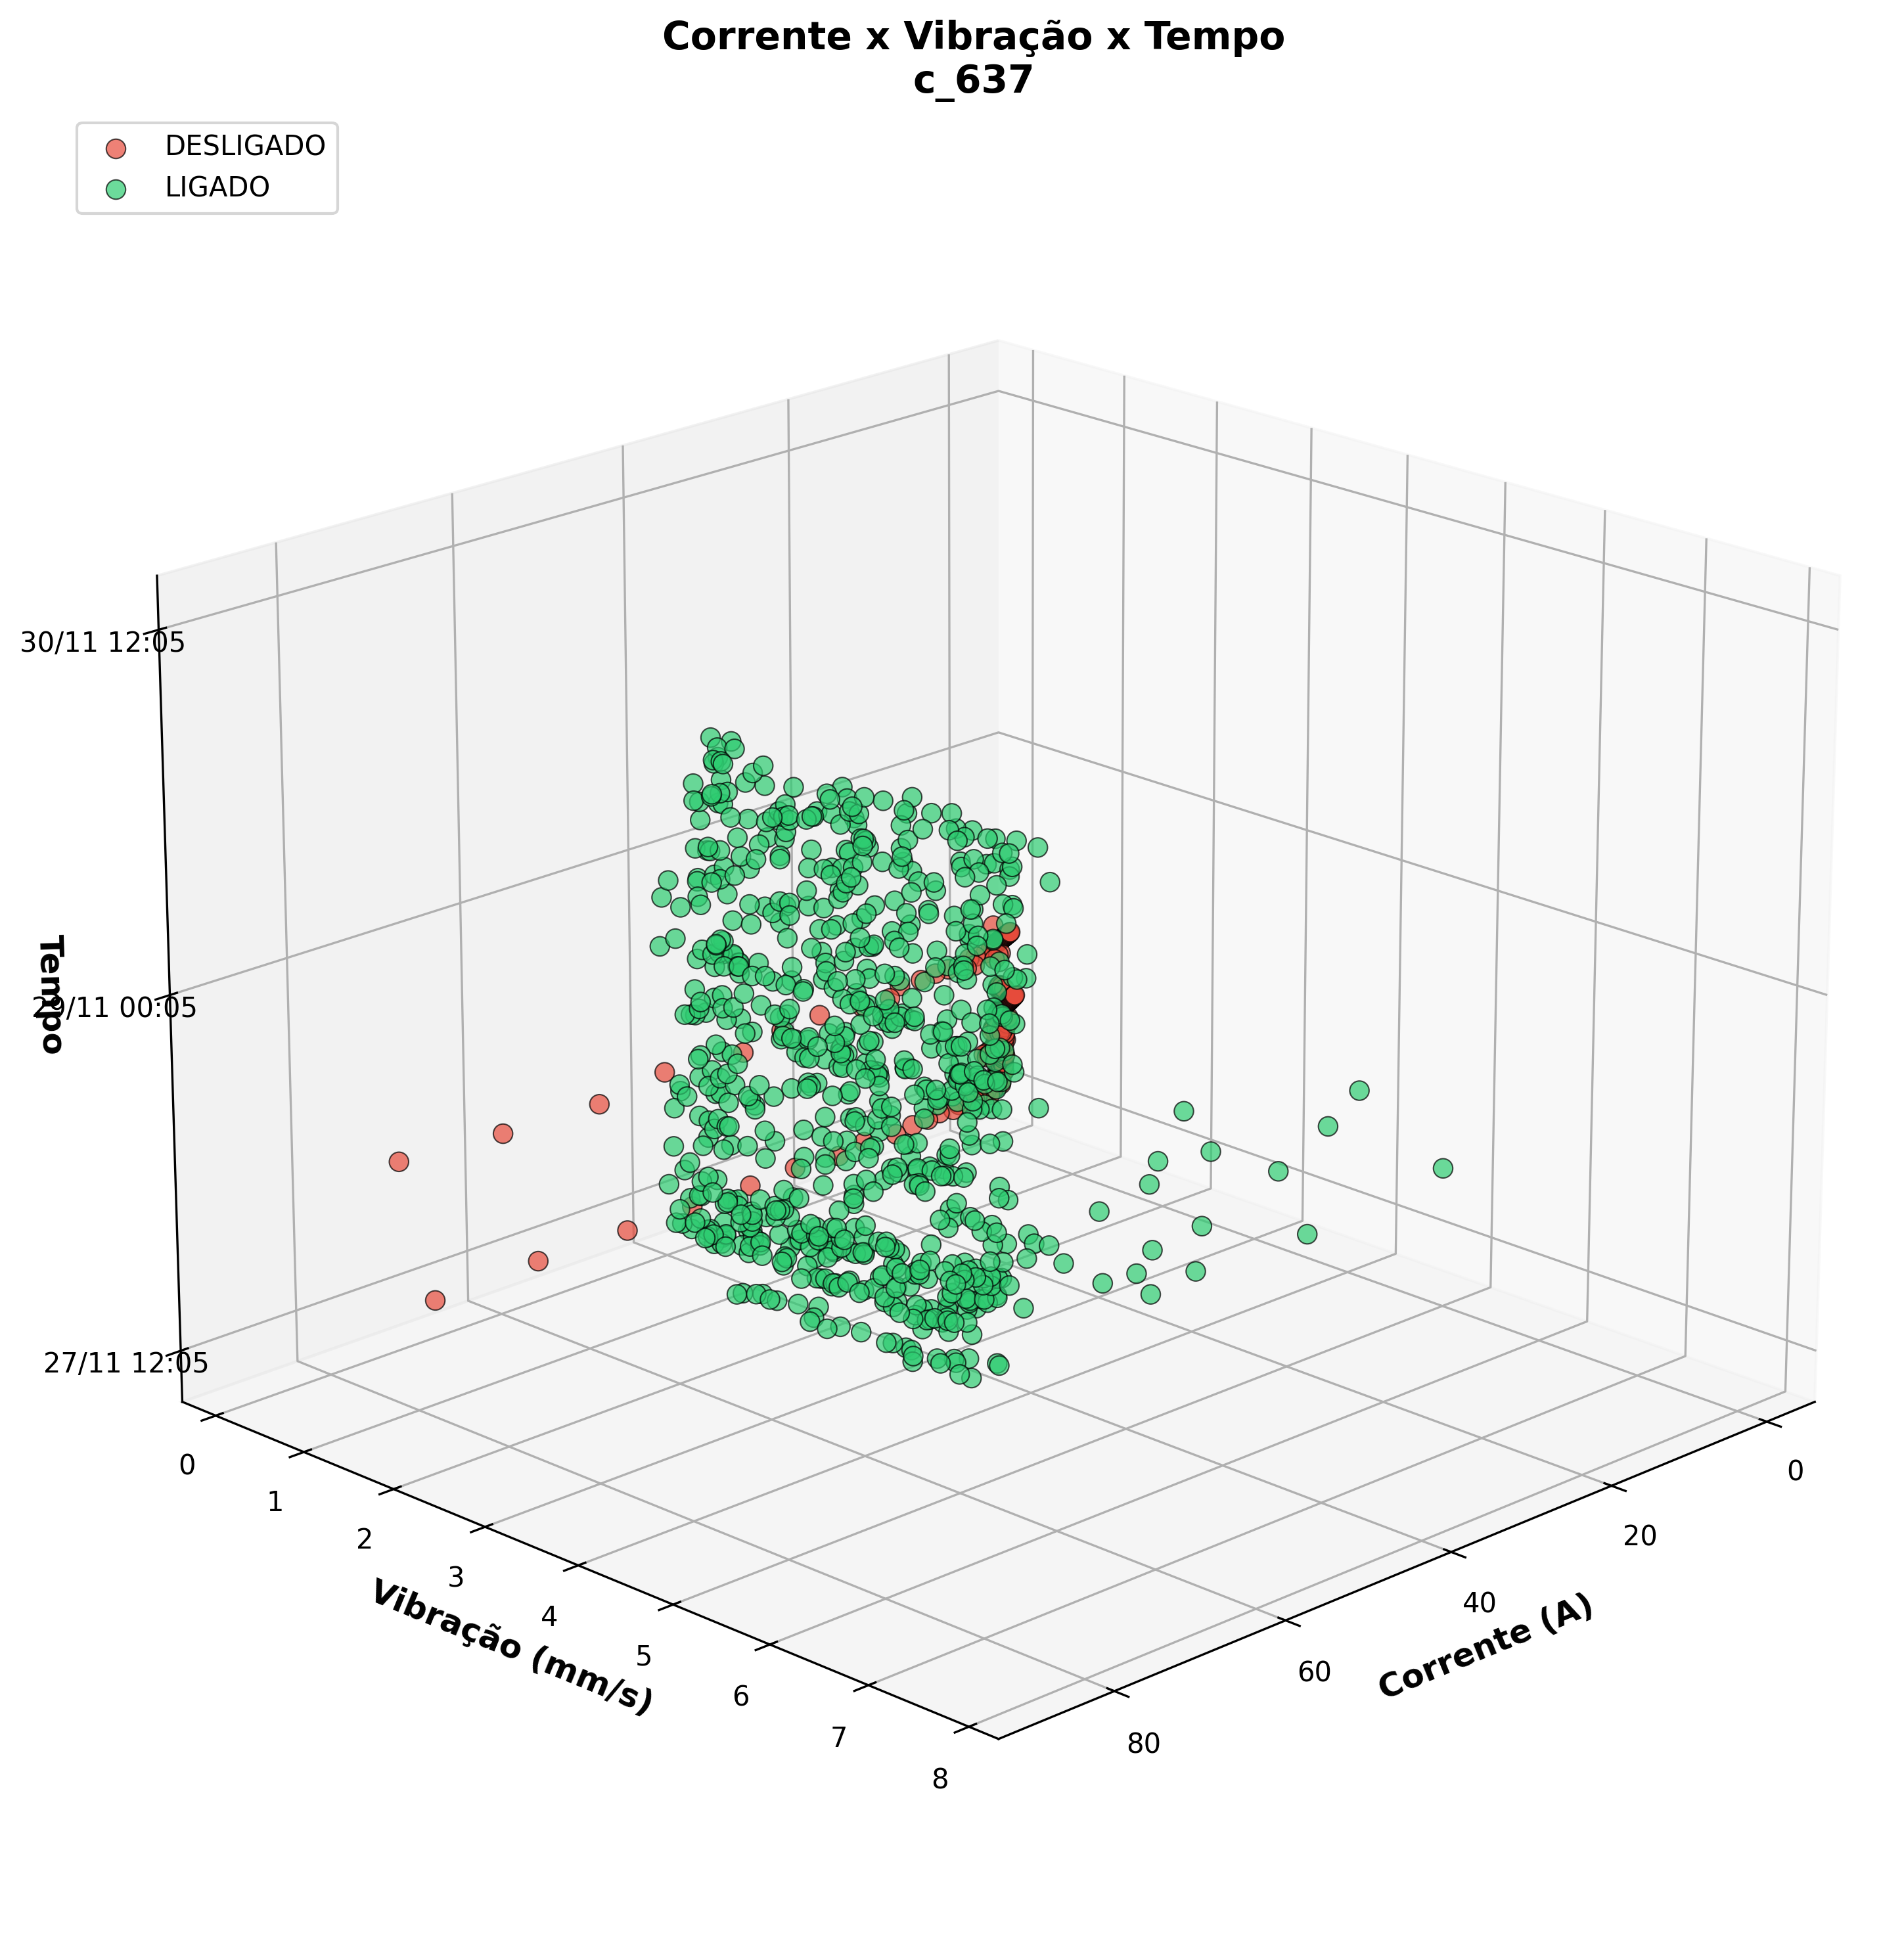
\includegraphics[width=0.7\textwidth]{results/estados_corrente_vibracao_tempo_3d_c_637.png}
    \caption{Visualização 3D -- Corrente $\times$ Vibração $\times$ Tempo -- Equipamento $c_{637}$. Demonstra a separação entre estados LIGADO (verde) e DESLIGADO (vermelho) ao longo do período histórico, com 1.242.993 amostras classificadas.}
    \label{fig:estados_3d_c_637_intervalo}
\end{figure}

O \textit{pipeline} implementa múltiplas estratégias de processamento com diferentes níveis de qualidade: dados originais sem interpolação (qualidade 1,00), interpolação PCHIP~\cite{fritsch1980pchip} para lacunas de até 30 minutos (qualidade 0,95) e interpolação KNN multivariada para lacunas entre 30 minutos e 3 horas (qualidade 0,75). Lacunas maiores que 3 horas resultam em segmentação automática em períodos distintos.

As visualizações 3D de \textit{clusters} utilizam redução de dimensionalidade por Análise de Componentes Principais (PCA) para projetar o espaço de 19 atributos (elétricos) ou 16 atributos (mecânicos) em dois eixos principais. O eixo PC1 (Componente Principal 1) captura a direção de máxima variância nos dados, tipicamente associada à distinção entre equipamento ligado e desligado. O eixo PC2 (Componente Principal 2) captura a segunda maior direção de variância, geralmente associada a diferenças entre regimes de operação (carga baixa \textit{versus} carga alta). Juntos, PC1 e PC2 permitem visualizar a separação entre estados de transição e estados estacionários do K-Means em um plano bidimensional.

\section{Análise de Dados Normalizados}

As Figuras~\ref{fig:dados_normalizados_c_636} a~\ref{fig:dados_normalizados_c_1518} apresentam a análise estatística dos dados após normalização MinMax com \textit{clipping} de \textit{outliers}, revelando a distribuição dos atributos normalizados e demonstrando a variabilidade dos sinais para cada equipamento.

A Figura~\ref{fig:dados_normalizados_c_636} apresenta a distribuição dos 19 atributos normalizados do equipamento $c_{636}$ (motobomba elétrica). Observa-se que o intervalo normalizado se estende de $-0,31$ a $1,29$, indicando a presença de valores levemente fora da faixa $[0,1]$ devido ao \textit{clipping} no percentil 99,5\%. O padrão revela corrente variável e RPM controlado, característicos de uma motobomba com ciclos de operação bem definidos.

\begin{figure}[H]
    \centering
    
\includegraphics[width=0.95\textwidth]{results/dados_normalizados_analise_c_636.png}
    \caption{Análise estatística dos dados normalizados -- Equipamento $c_{636}$. Distribuição dos 19 atributos após normalização MinMax com intervalo $[-0,31;\ 1,29]$, revelando padrões característicos de operação com corrente variável e RPM controlado.}
    \label{fig:dados_normalizados_c_636}
\end{figure}

A Figura~\ref{fig:dados_normalizados_c_637} exibe os dados normalizados do equipamento $c_{637}$ (motobomba elétrica). Diferentemente do $c_{636}$, este equipamento apresenta distribuição uniforme dos 19 atributos no intervalo $[0,0;\ 1,0]$, indicando operação mais estável e menor variabilidade de corrente.

\begin{figure}[H]
    \centering
    
\includegraphics[width=0.6\textwidth]{results/dados_normalizados_analise_c_637.png}
    \caption{Análise estatística dos dados normalizados -- Equipamento $c_{637}$. Distribuição uniforme dos 19 atributos no intervalo $[0,0;\ 1,0]$, indicando operação mais estável com menor variabilidade de corrente.}
    \label{fig:dados_normalizados_c_637}
\end{figure}

A Figura~\ref{fig:dados_normalizados_c_640} mostra os dados normalizados do equipamento $c_{640}$ (Motor REC). Nota-se forte concentração em valores baixos na maioria dos atributos, o que é característico de um equipamento com longos períodos de desligamento (69\% do tempo no estado DESLIGADO, conforme será detalhado na Seção~4.4).

\begin{figure}[H]
    \centering
    
\includegraphics[width=0.6\textwidth]{results/dados_normalizados_analise_c_640.png}
    \caption{Análise estatística dos dados normalizados -- Equipamento $c_{640}$. Distribuição dos 19 atributos com forte concentração em valores baixos, característico de equipamento com longos períodos de desligamento.}
    \label{fig:dados_normalizados_c_640}
\end{figure}

A Figura~\ref{fig:dados_normalizados_c_670} apresenta os dados normalizados do equipamento mecânico $c_{670}$ (redutora \textit{bridle}). Utiliza-se um conjunto reduzido de 16 atributos específicos para equipamentos mecânicos, com ênfase em temperatura e vibração como indicadores principais do estado operacional.

\begin{figure}[H]
    \centering
    
\includegraphics[width=0.6\textwidth]{results/dados_normalizados_analise_c_670_mecanico.png}
    \caption{Análise estatística dos dados normalizados -- Equipamento $c_{670}$ (mecânico). Distribuição dos 16 atributos específicos para equipamentos mecânicos, com ênfase em temperatura e vibração.}
    \label{fig:dados_normalizados_c_670}
\end{figure}

Por fim, a Figura~\ref{fig:dados_normalizados_c_1518} exibe a distribuição normalizada do equipamento mecânico $c_{1518}$ (mancal). Os padrões distintos de temperatura e vibração revelam operação intermitente, com transições frequentes entre estados ligado e desligado.

\begin{figure}[H]
    \centering
    
\includegraphics[width=0.6\textwidth]{results/dados_normalizados_analise_c_1518_mecanico.png}
    \caption{Análise estatística dos dados normalizados -- Equipamento $c_{1518}$ (mecânico). Distribuição dos 16 atributos mecânicos, revelando padrões distintos de temperatura e vibração característicos de operação intermitente.}
    \label{fig:dados_normalizados_c_1518}
\end{figure}
\vspace{-0.3cm}

\section{Resultados da Clusterização K-Means}

O algoritmo K-Means foi executado com $k = 6$ \textit{clusters} para todos os equipamentos, mostrando convergência robusta. A escolha de $k = 6$ foi motivada pela necessidade de representar a proporção aproximada de 1 para 2 entre estados desligado e ligado: com 6 \textit{clusters}, garante-se a existência de pelo menos um \textit{cluster} que represente inequivocamente o estado DESLIGADO, pelo menos um que represente um estado de transição (desligando ou ligando, ou seja, estados intermediários entre os dois extremos), e os restantes representando diferentes regimes de operação LIGADO sob cargas variáveis. Essa proporção assegura que o sistema não confunda estados transitórios com estados estacionários, melhorando a robustez da classificação final.

As inércias finais variaram entre cerca de 127 e 178 mil, indicando que os \textit{clusters} formados apresentaram baixa dispersão interna, ou seja, os pontos dentro de cada \textit{cluster} estavam próximos entre si. O tempo de processamento foi de 1 a 2 minutos por equipamento, utilizando um notebook Dell equipado com processador Intel Core i3 de 13\textsuperscript{a} geração e 64 GB de memória RAM. A acurácia máxima de classificação e reprodutibilidade foram garantidas através de \textit{random state} controlado. A classificação dinâmica baseada em \textit{scores} combinados identificou automaticamente \textit{clusters} LIGADO e DESLIGADO.

A distribuição automática dos estados DESLIGADO e LIGADO para cada equipamento está apresentada na Tabela~\ref{tab:distribuicao_estados}. A análise dos centróides mostrou que os \textit{clusters} DESLIGADO apresentam valores baixos de magnetômetro, temperatura e vibração normalizados, enquanto os \textit{clusters} LIGADO apresentam valores elevados, refletindo claramente os diferentes estados operacionais de cada equipamento, desde motobombas até componentes mecânicos.

\begin{table}[H]
    \centering
    \caption{Distribuição dos estados DESLIGADO e LIGADO por equipamento}
    \label{tab:distribuicao_estados}
    \begin{tabular}{lcc}
        \hline
        Equipamento & DESLIGADO (\%) & LIGADO (\%) \\
        \hline
        $c_{636}$   & 4,75           & 95,25       \\
        $c_{637}$   & 4,52           & 95,48       \\
        $c_{640}$   & 5,64           & 94,36       \\
        $c_{1518}$  & 4,76           & 95,24       \\
        $c_{670}$   & 20,99          & 79,01       \\
        \hline
    \end{tabular}
\end{table}

\section{Visualização dos \textit{Clusters}}

As visualizações 3D a seguir mostram a distribuição espacial dos 6 \textit{clusters} K-Means no espaço de atributos, permitindo interpretação visual da separabilidade entre estados LIGADO e DESLIGADO dos equipamentos elétricos (motobombas e motor) e mecânicos (mancal e redutora).

A Figura~\ref{fig:analise_clusters_c_636} apresenta os \textit{clusters} do equipamento $c_{636}$ (motobomba elétrica), onde se observa separação clara entre o \textit{cluster} DESLIGADO (em vermelho) e os \textit{clusters} LIGADO (em verde), com fronteira bem definida no espaço tridimensional.

\begin{figure}[H]
    \centering
    
\includegraphics[width=0.65\textwidth]{results/analise_kmeans_clusters_moderado_c_636.png}
    \caption{\textit{Clusters} K-Means 3D -- $c_{636}$. Separação clara entre DESLIGADO (vermelho) e LIGADO (verde).}
    \label{fig:analise_clusters_c_636}
\end{figure}

A Figura~\ref{fig:analise_clusters_c_637} mostra os \textit{clusters} do equipamento $c_{637}$ (motobomba elétrica), com um \textit{cluster} classificado como DESLIGADO (4,52\%) e cinco como LIGADO (95,48\%), com inércia final de 138.139.

\begin{figure}[H]
    \centering
    
\includegraphics[width=0.65\textwidth]{results/analise_kmeans_clusters_moderado_c_637.png}
    \caption{\textit{Clusters} K-Means 3D -- $c_{637}$. Um \textit{cluster} DESLIGADO (4,52\%) e cinco LIGADO (95,48\%), com 1.242.993 amostras.}
    \label{fig:analise_clusters_c_637}
\end{figure}

A Figura~\ref{fig:analise_clusters_c_640} exibe os \textit{clusters} do equipamento $c_{640}$ (Motor REC), com um \textit{cluster} DESLIGADO (5,64\%) e cinco LIGADO (94,36\%), com inércia final de 125.670.

\begin{figure}[H]
    \centering
    
\includegraphics[width=0.65\textwidth]{results/analise_kmeans_clusters_moderado_c_640.png}
    \caption{\textit{Clusters} K-Means 3D -- $c_{640}$. Um \textit{cluster} DESLIGADO (5,64\%) e distribuição equilibrada dos cinco LIGADO, com 1.389.174 amostras.}
    \label{fig:analise_clusters_c_640}
\end{figure}

A Figura~\ref{fig:analise_clusters_c_1518} apresenta os \textit{clusters} do equipamento mecânico $c_{1518}$ (mancal), cuja classificação é baseada em temperatura e vibração. Com apenas 4,76\% do tempo em estado DESLIGADO, este equipamento demonstra operação quase contínua.

\begin{figure}[H]
    \centering
    
\includegraphics[width=0.65\textwidth]{results/analise_kmeans_clusters_mecanico_c_1518.png}
    \caption{\textit{Clusters} K-Means 3D -- $c_{1518}$. Classificação baseada em temperatura e vibração para equipamento mecânico (Mancal), com 4,76\% DESLIGADO e 585.367 amostras.}
    \label{fig:analise_clusters_c_1518}
\end{figure}

Por fim, a Figura~\ref{fig:analise_clusters_c_670} mostra os \textit{clusters} do equipamento mecânico $c_{670}$ (redutora \textit{bridle}), com separação binária clara entre DESLIGADO e LIGADO baseada exclusivamente em dados mecânicos (temperatura e vibração), sem necessidade de corrente ou RPM.

\begin{figure}[H]
    \centering
    
\includegraphics[width=0.65\textwidth]{results/analise_kmeans_clusters_mecanico_c_670.png}
    \caption{\textit{Clusters} K-Means 3D -- $c_{670}$. Separação binária entre DESLIGADO (20,99\%) e LIGADO (79,01\%) baseada em dados mecânicos, com 1.377.884 amostras.}
    \label{fig:analise_clusters_c_670}
\end{figure}
\vspace{-0.3cm}

\section{Visualizações 3D de Estados Operacionais}

O \textit{pipeline} K-Means permite gerar visualizações tridimensionais automáticas que mostram a evolução temporal dos estados operacionais dos equipamentos. Essas visualizações ajudam a compreender a dinâmica entre variáveis como corrente, RPM, temperatura e vibração, destacando os estados LIGADO e DESLIGADO ao longo do tempo. É possível analisar tanto períodos históricos quanto intervalos específicos com dados atuais, obtidos em tempo real via InfluxDB, facilitando o diagnóstico de padrões operacionais e a validação do \textit{pipeline} com dados recentes não utilizados no treinamento.

A Figura~\ref{fig:3d_corrente_c636} apresenta o espaço Corrente $\times$ Vibração $\times$ Tempo do equipamento $c_{636}$ ao longo do período histórico completo. Os pontos em verde representam o estado LIGADO, concentrados em regiões de alta corrente e vibração, enquanto os pontos em vermelho (DESLIGADO) agrupam-se próximos à origem, confirmando a separação eficaz dos estados.

\begin{figure}[H]
    \centering
    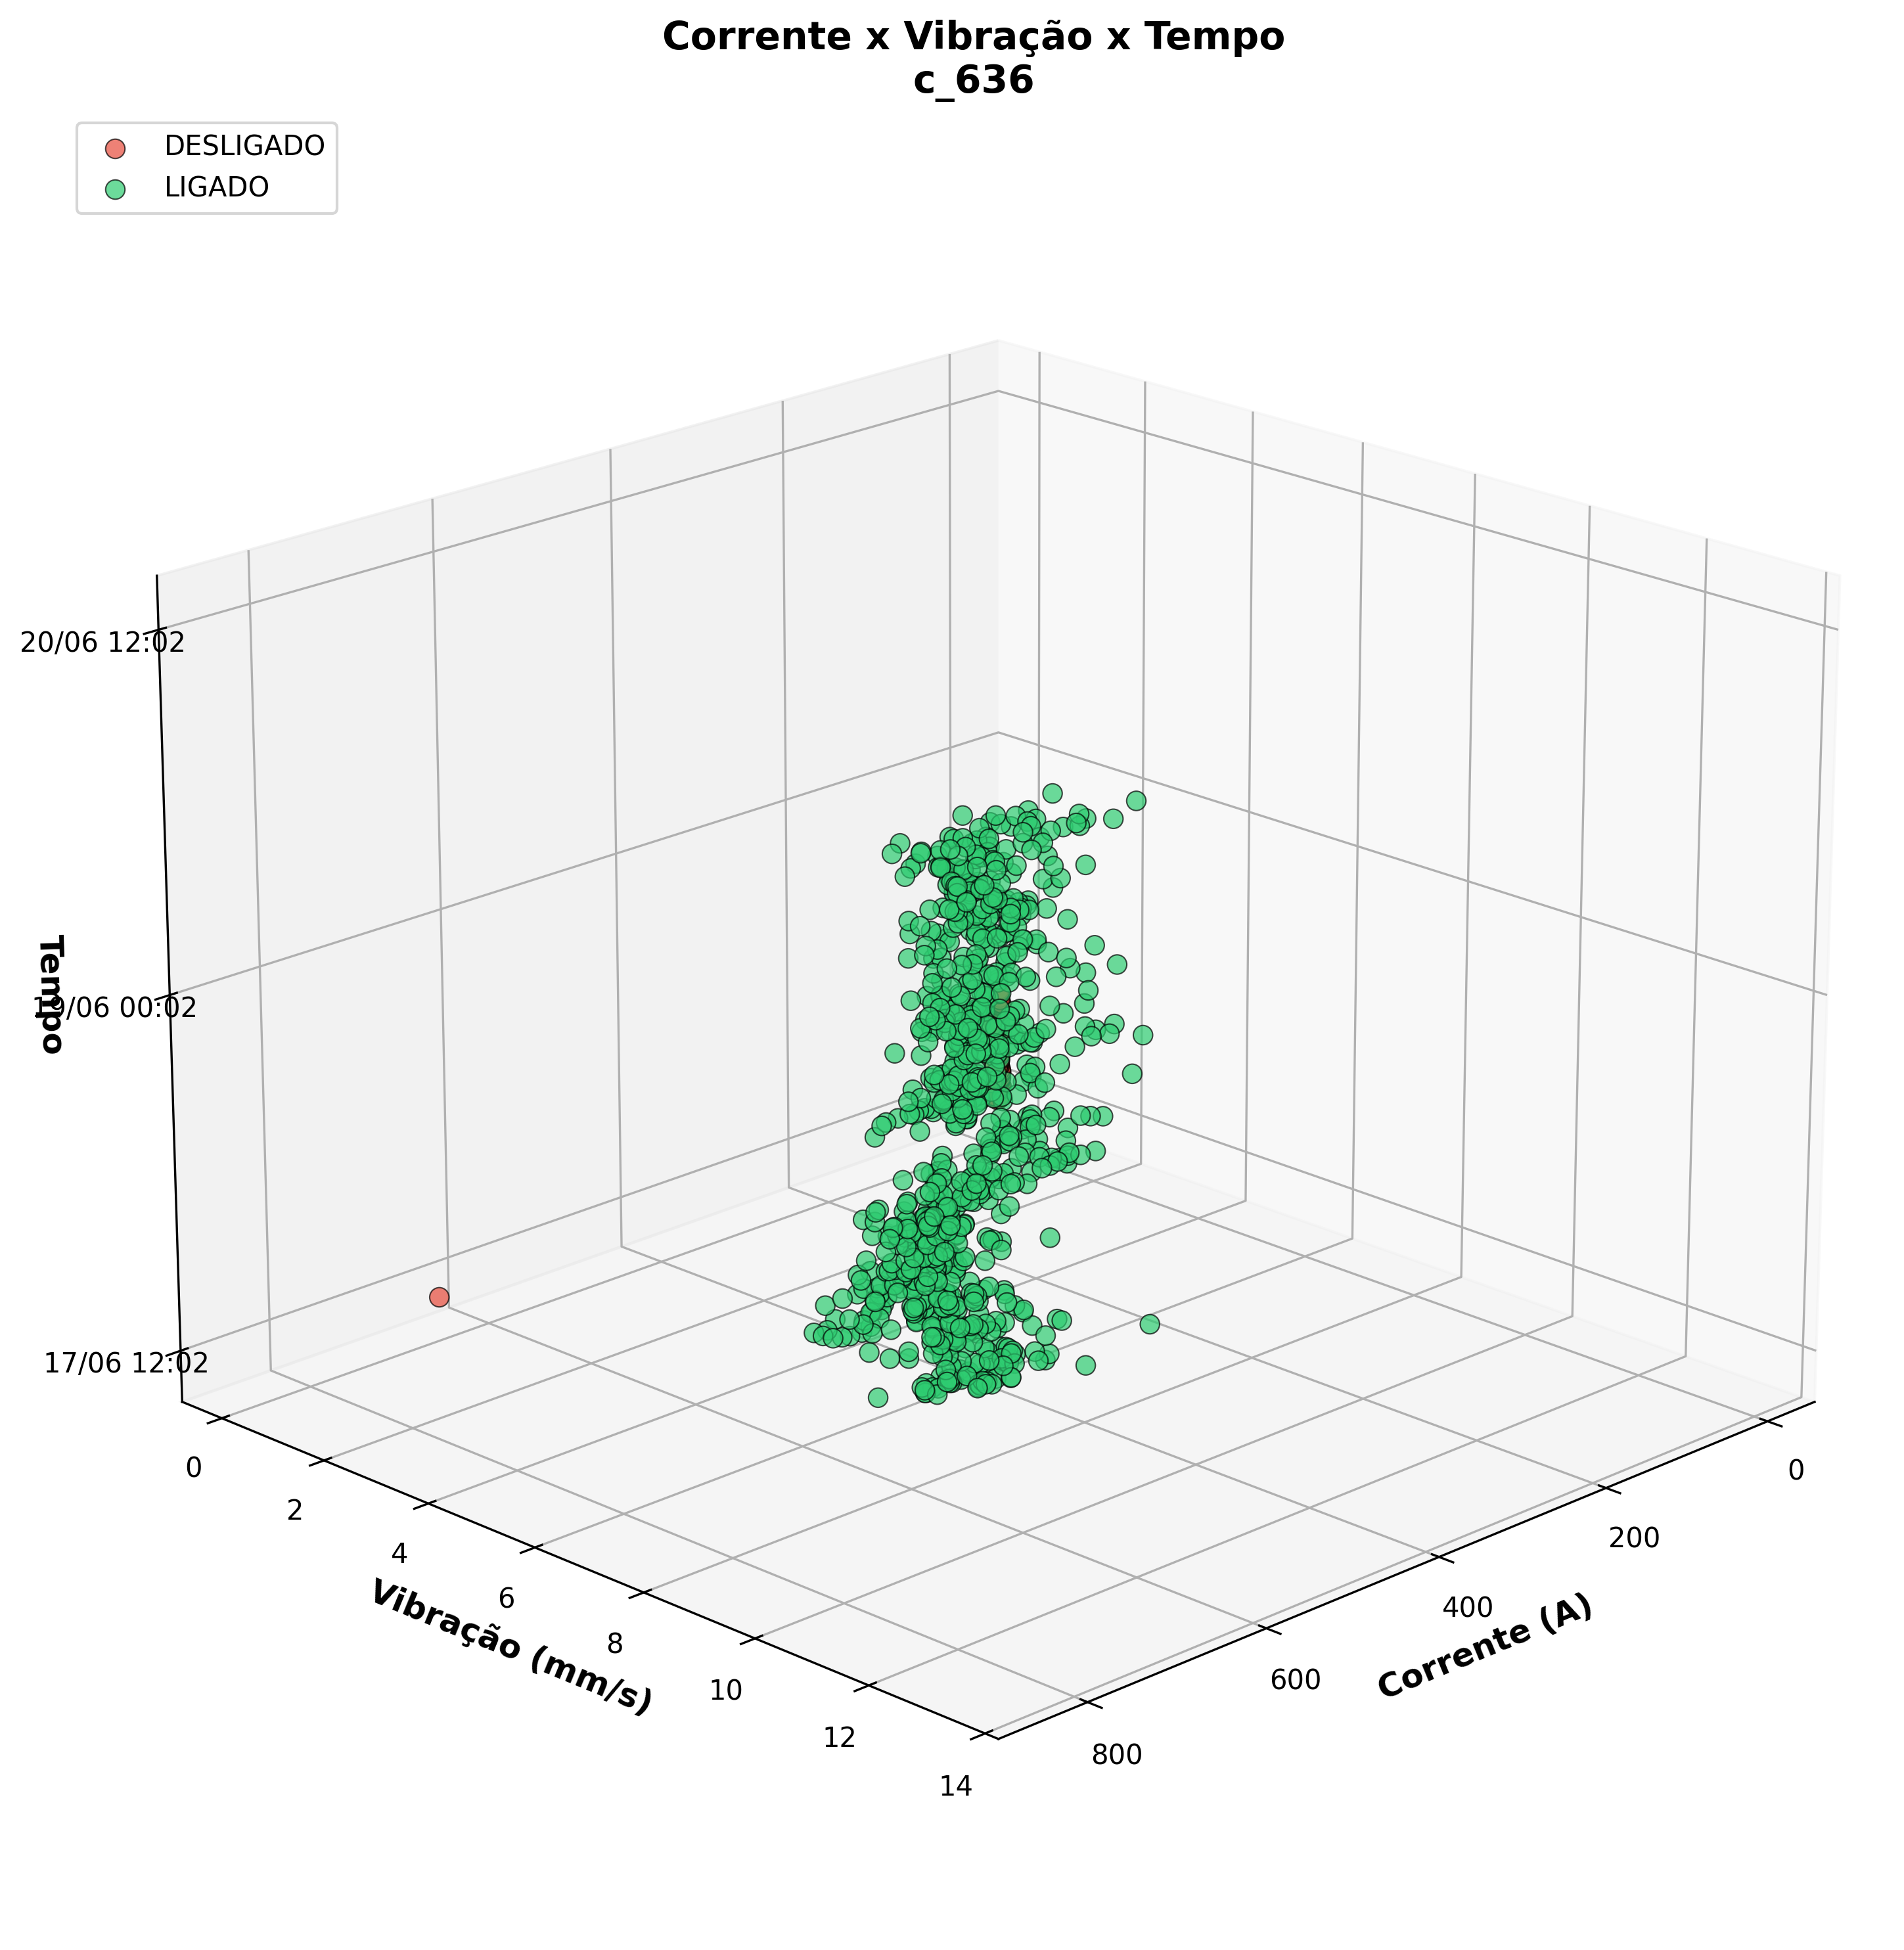
\includegraphics[width=0.55\textwidth]{results/estados_corrente_vibracao_tempo_3d_c_636.png}
    \caption{Corrente $\times$ Vibração $\times$ Tempo -- $c_{636}$, período histórico. Verde: LIGADO, vermelho: DESLIGADO.}
    \label{fig:3d_corrente_c636}
\end{figure}

A Figura~\ref{fig:3d_rpm_c636} mostra o espaço RPM $\times$ Vibração $\times$ Tempo para o mesmo equipamento $c_{636}$. Observa-se forte correlação entre velocidade rotacional e vibração: quando o RPM é elevado, a vibração acompanha proporcionalmente, validando a coerência física da classificação.

\begin{figure}[H]
    \centering
    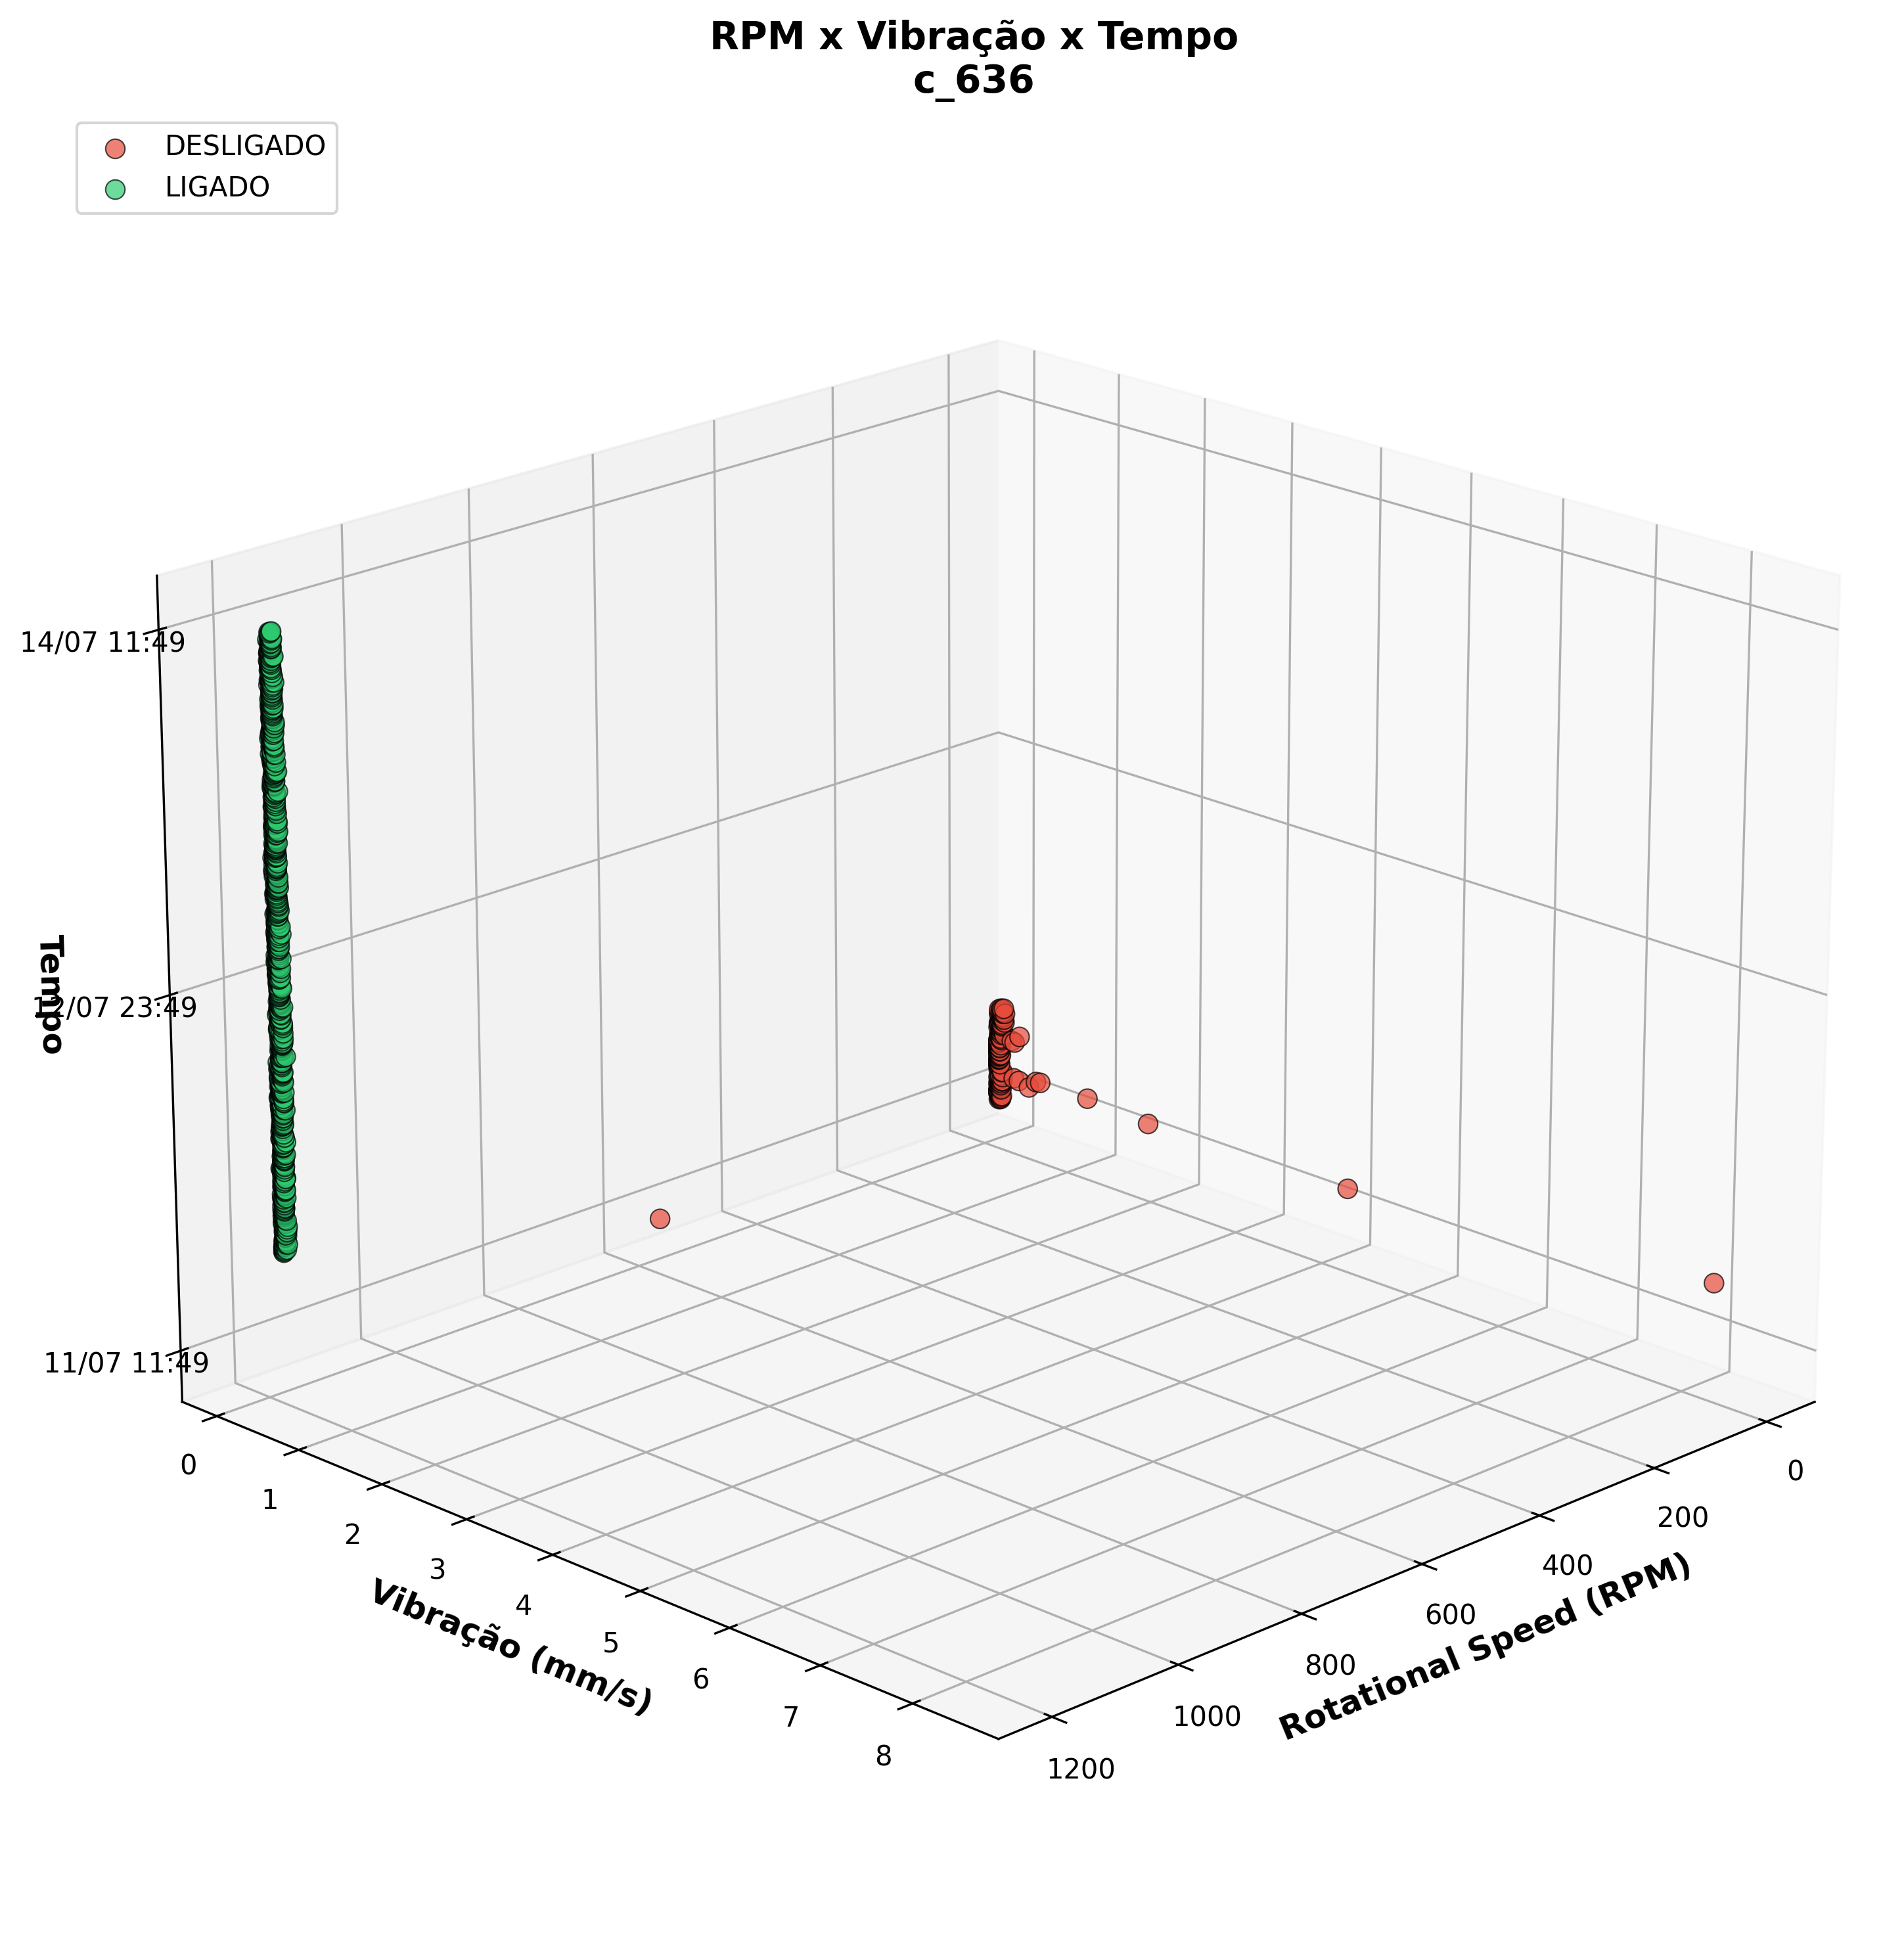
\includegraphics[width=0.55\textwidth]{results/estados_rpm_vibracao_tempo_3d_c_636.png}
    \caption{RPM $\times$ Vibração $\times$ Tempo -- $c_{636}$, período histórico. Correlação entre velocidade rotacional e vibração.}
    \label{fig:3d_rpm_c636}
\end{figure}

A Figura~\ref{fig:3d_corrente_c637} exibe o espaço Corrente $\times$ Vibração $\times$ Tempo do equipamento $c_{637}$, com 4,52\% do tempo em DESLIGADO.

\begin{figure}[H]
    \centering
    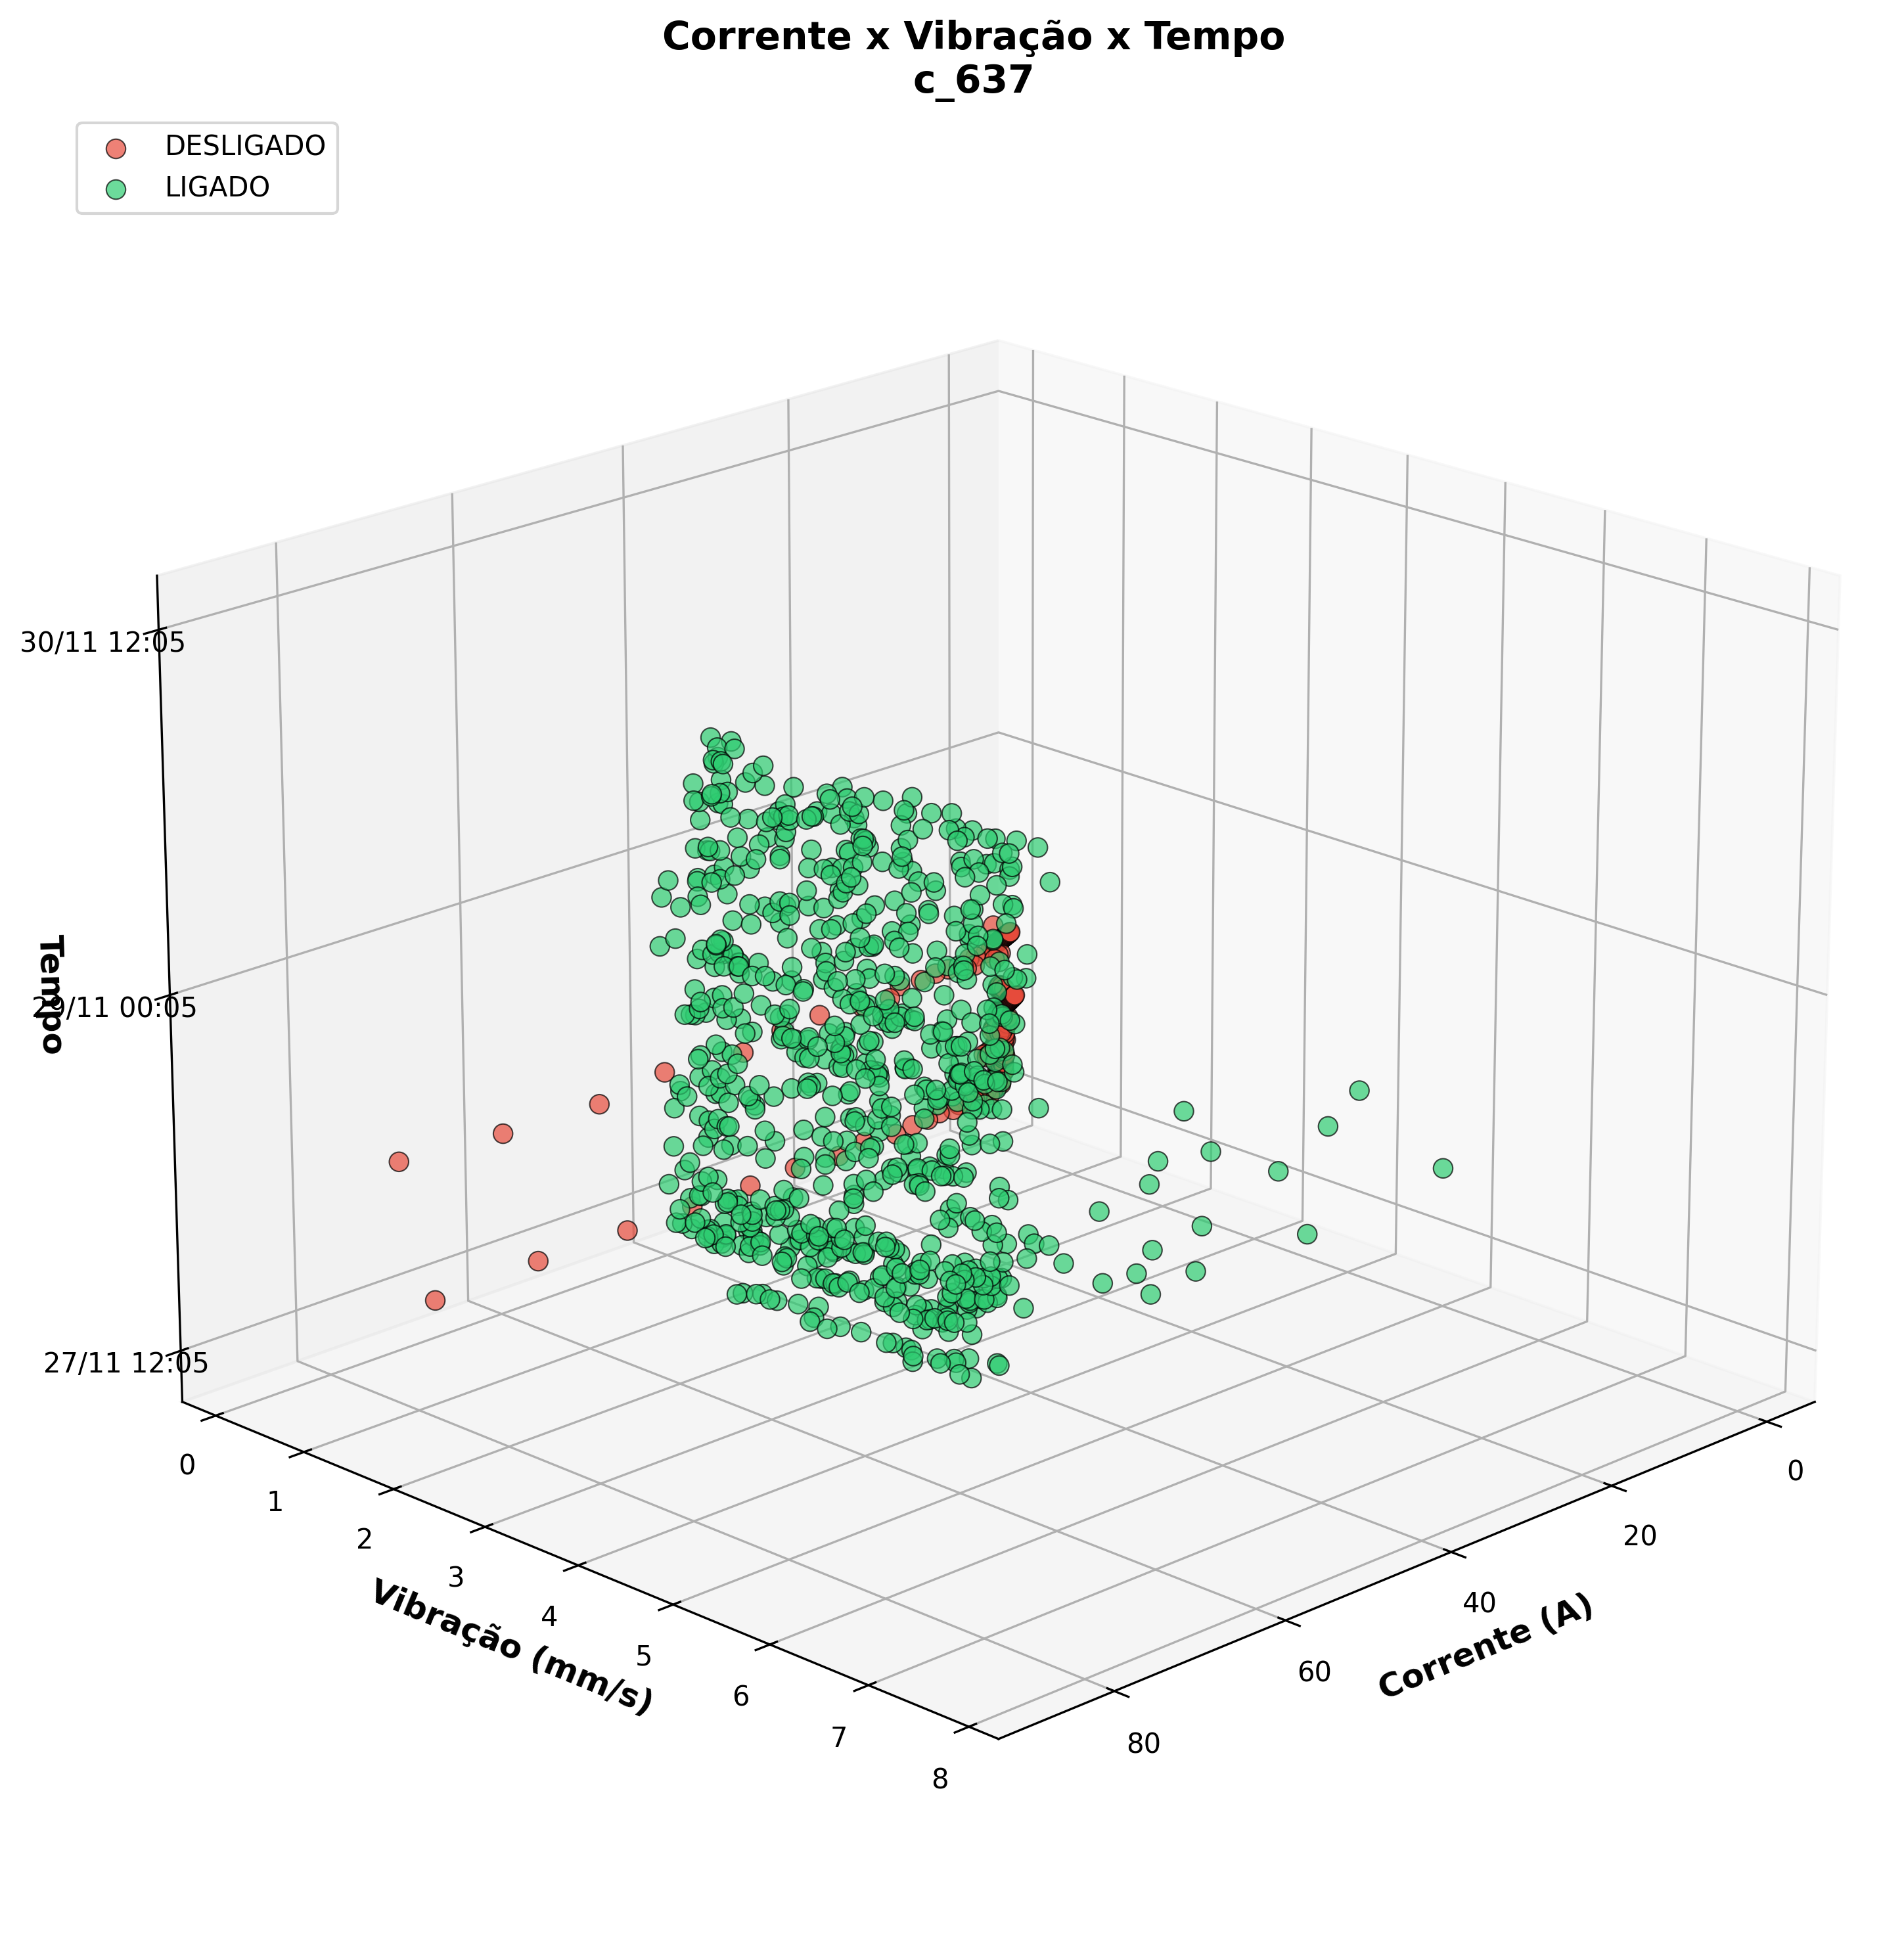
\includegraphics[width=0.95\textwidth]{results/estados_corrente_vibracao_tempo_3d_c_637.png}
    \caption{Corrente $\times$ Vibração $\times$ Tempo -- $c_{637}$, período histórico. 95,48\% LIGADO e 4,52\% DESLIGADO.}
    \label{fig:3d_corrente_c637}
\end{figure}

A Figura~\ref{fig:3d_rpm_c637} apresenta o espaço RPM $\times$ Vibração $\times$ Tempo do equipamento $c_{637}$, onde se identificam dois \textit{clusters} DESLIGADO distintos e múltiplos \textit{clusters} LIGADO, revelando diferentes regimes de velocidade durante a operação.

\begin{figure}[H]
    \centering
    
\includegraphics[width=0.95\textwidth]{results/estados_rpm_vibracao_tempo_3d_c_637.png}
    \caption{RPM $\times$ Vibração $\times$ Tempo -- $c_{637}$, período histórico. Dois \textit{clusters} DESLIGADO e múltiplos LIGADO.}
    \label{fig:3d_rpm_c637}
\end{figure}

A Figura~\ref{fig:3d_corrente_c640} mostra o espaço Corrente $\times$ Vibração $\times$ Tempo do equipamento $c_{640}$ (Motor REC). Com 5,64\% do tempo em estado DESLIGADO e 94,36\% LIGADO.

\begin{figure}[H]
    \centering
    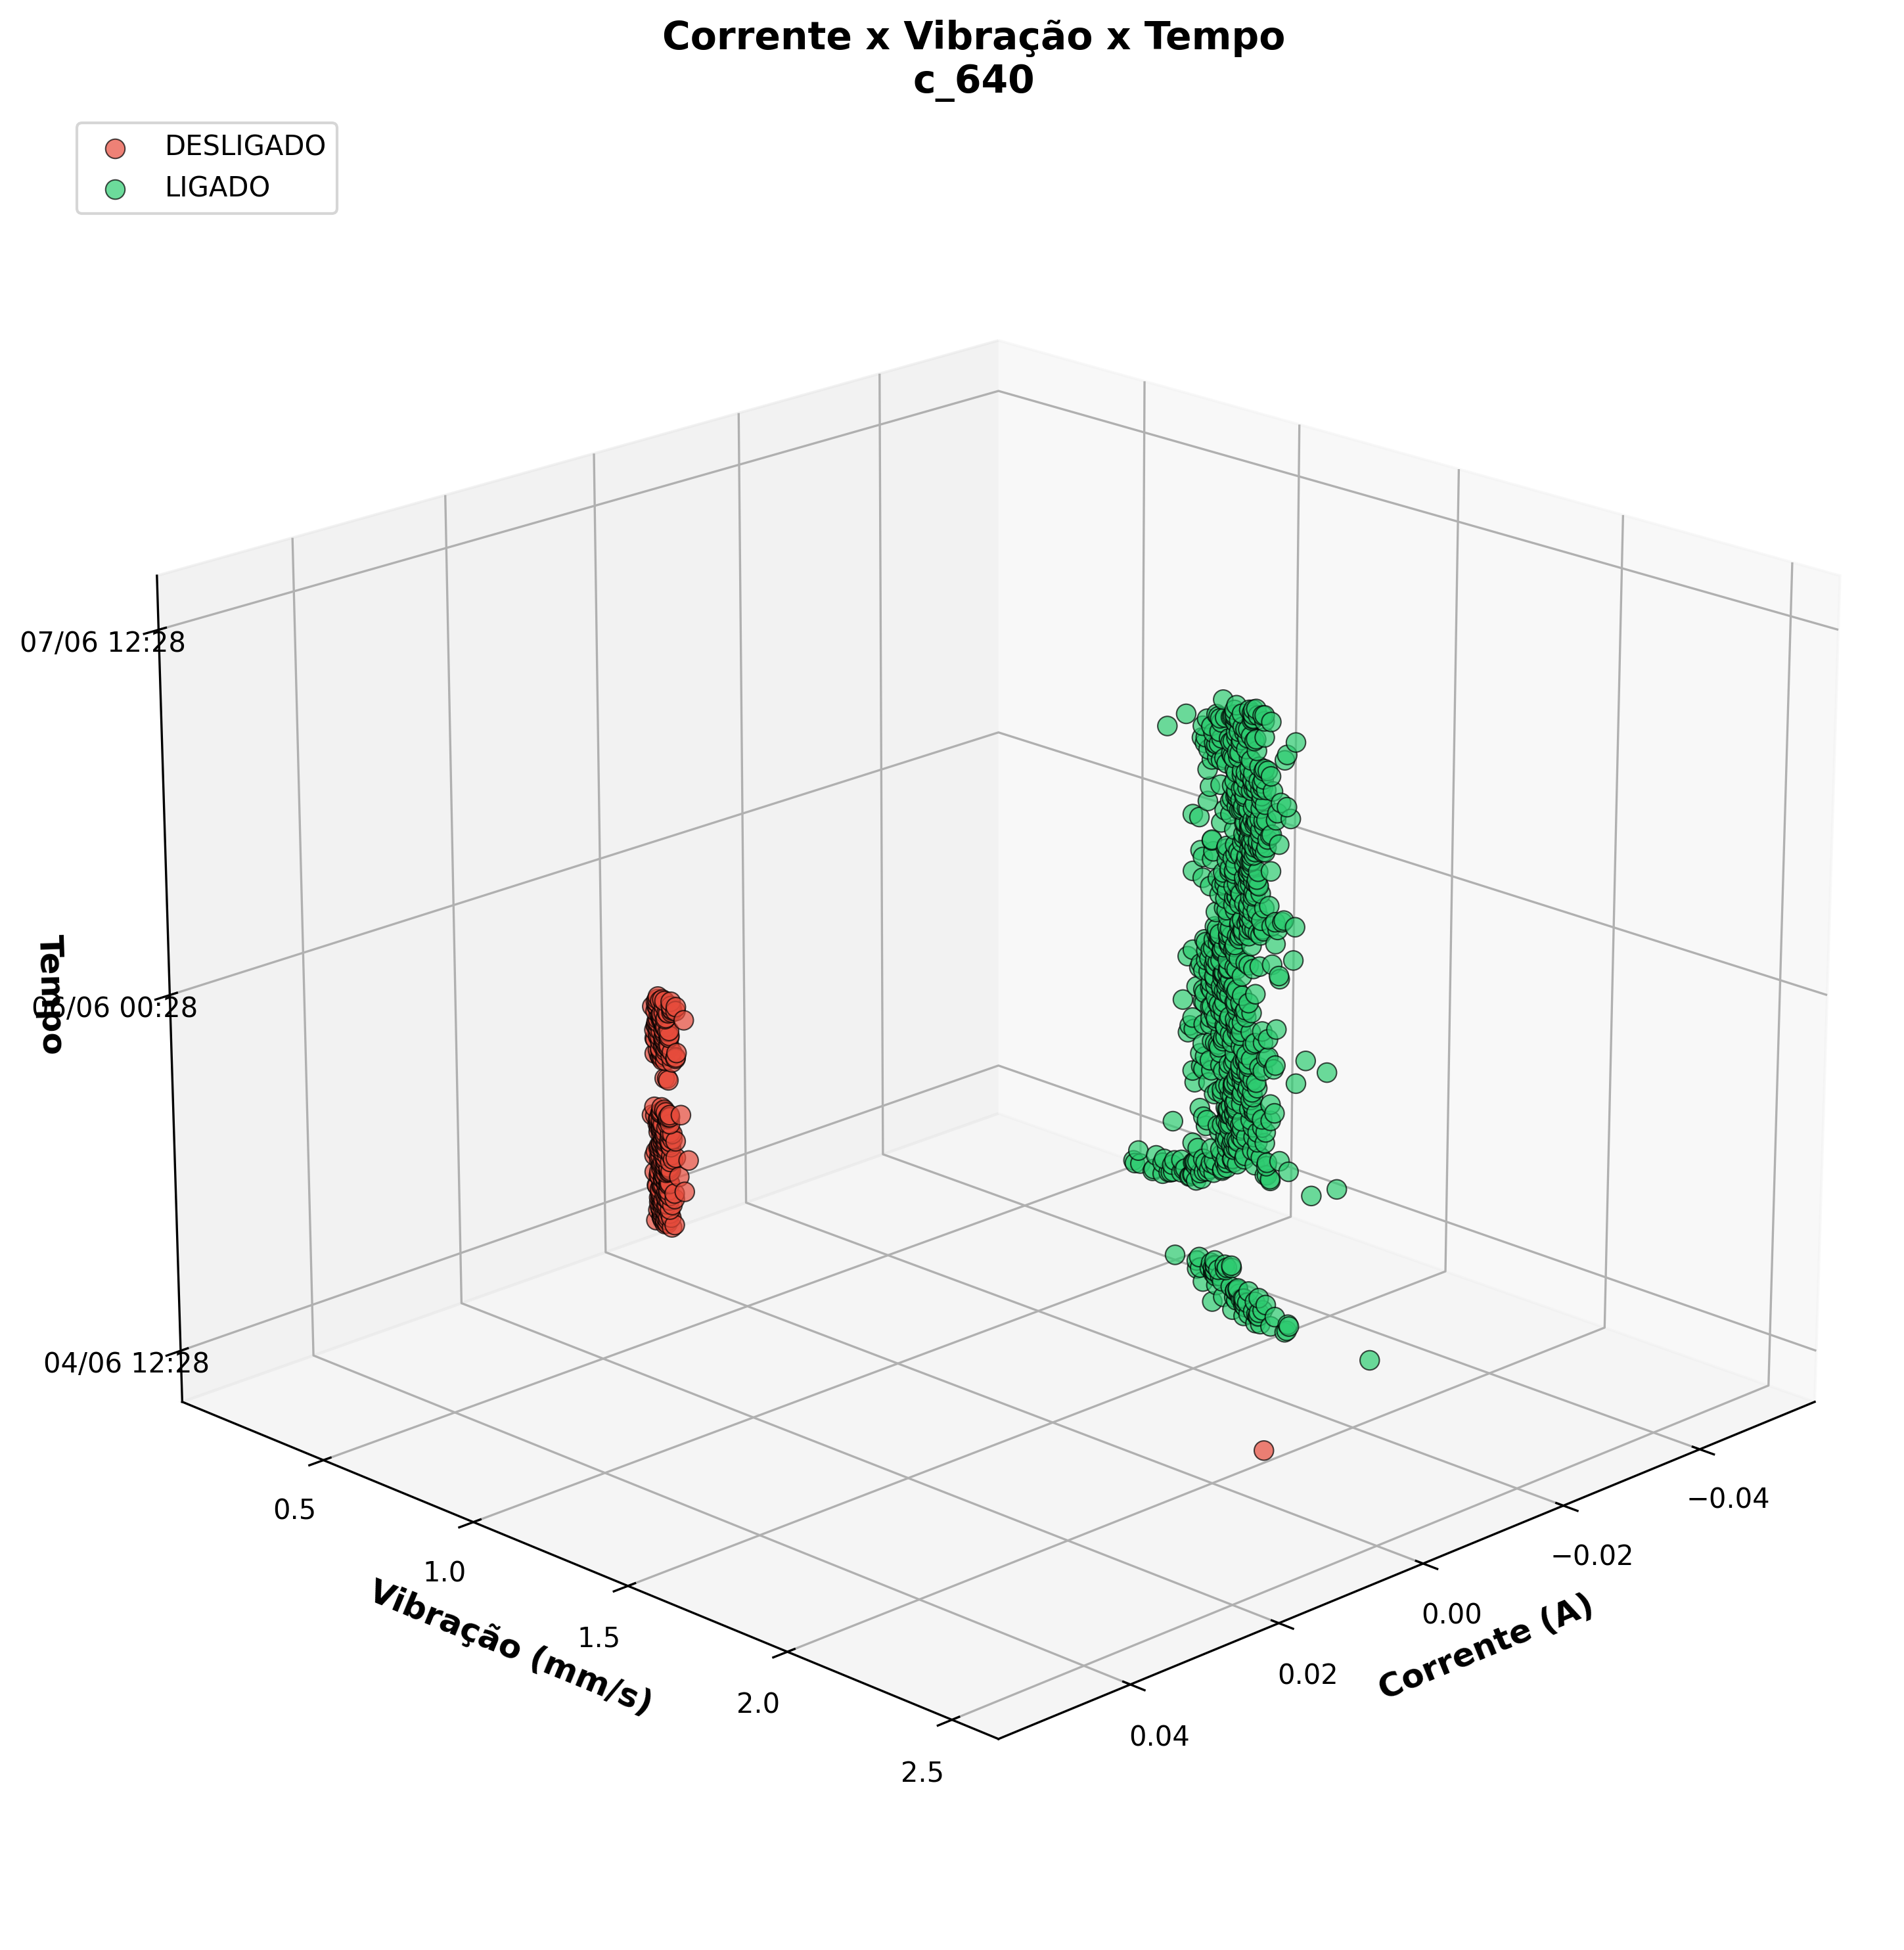
\includegraphics[width=0.55\textwidth]{results/estados_corrente_vibracao_tempo_3d_c_640.png}
    \caption{Corrente $\times$ Vibração $\times$ Tempo -- $c_{640}$, período histórico. 94,36\% LIGADO e 5,64\% DESLIGADO.}
    \label{fig:3d_corrente_c640}
\end{figure}

Por fim, a Figura~\ref{fig:3d_rpm_c640} exibe o espaço RPM $\times$ Vibração $\times$ Tempo do equipamento $c_{640}$, evidenciando distribuição equilibrada dos \textit{clusters} LIGADO em diferentes faixas de RPM, o que indica operação em múltiplos regimes de velocidade.

\begin{figure}[H]
    \centering
    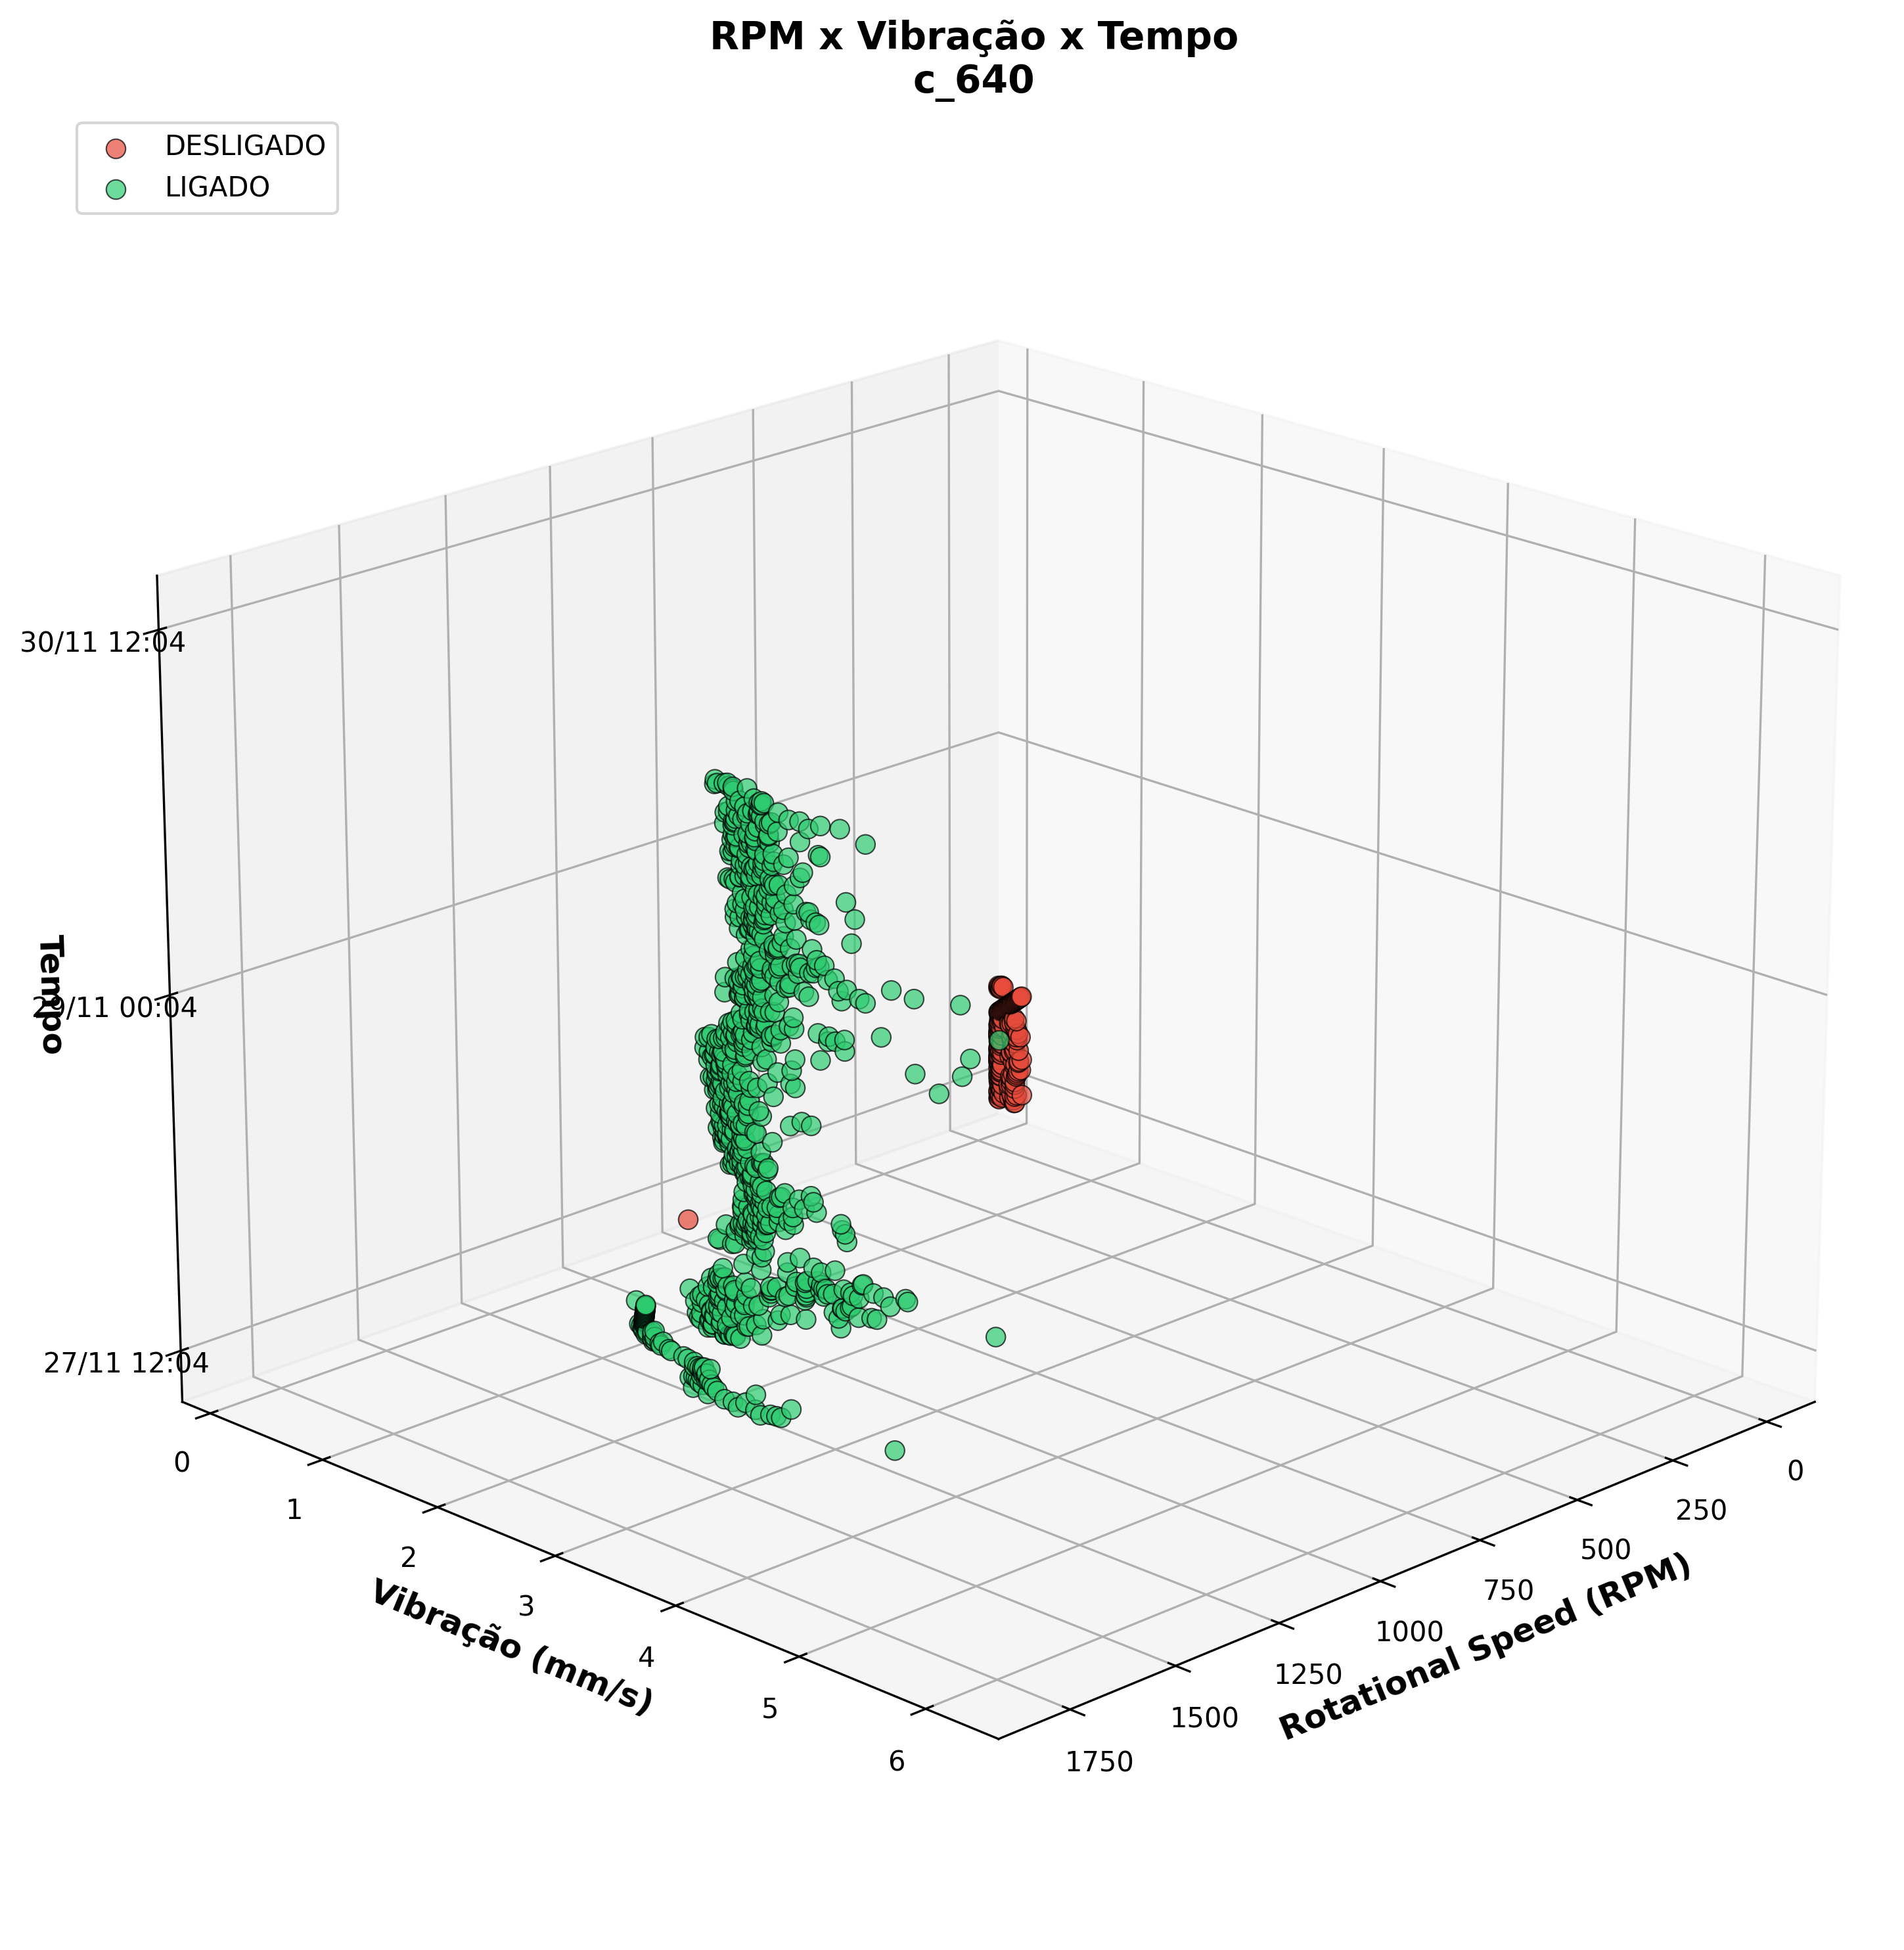
\includegraphics[width=0.6\textwidth]{results/estados_rpm_vibracao_tempo_3d_c_640.png}
    \caption{RPM $\times$ Vibração $\times$ Tempo -- $c_{640}$, período histórico. Distribuição equilibrada de \textit{clusters} LIGADO.}
    \label{fig:3d_rpm_c640}
\end{figure}

A Tabela~\ref{tab:validacao_classificacao} resume os métodos de validação empregados e suas respectivas observações, confirmando a consistência total e alta confiabilidade da classificação automática.

\begin{table}[H]
    \centering
    \caption{Validação da classificação automática}
    \label{tab:validacao_classificacao}
    \begin{tabular}{|l|l|}
        \hline
        Método de Validação      & Observações                           \\
        \hline
        Classificação automática & Baseada em \textit{scores} combinados \\
        Consistência temporal    & Transições suaves detectadas          \\
        Separação visual         & \textit{Clusters} bem definidos       \\
        Reprodutibilidade        & Mesmo resultado em re-execuções       \\
        \hline
    \end{tabular}
\end{table}

O \textit{pipeline} de treinamento implementa validações automáticas rigorosas aplicadas exclusivamente à fase de aprendizado. Ele rejeita períodos com lacunas superiores a 3 horas ou dados insuficientes (menos de 24 horas) para garantir que os centróides do K-Means sejam calculados sobre ciclos operacionais íntegros. Já na etapa de classificação de intervalos, o sistema processa 100\% dos pontos do período solicitado, visando a reconstrução total dos dados. O \textit{pipeline} monitora a eficiência de processamento entre 30 e 100\% para assegurar a qualidade dos dados e realiza verificação automática da acurácia de classificação. Essa abordagem conservadora prioriza precisão na modelagem, assegurando resultados consistentes e confiáveis na predição.
\vspace{-0.3cm}

\section{Desempenho Computacional}

A Tabela~\ref{tab:tempos_execucao} apresenta o tempo de execução de cada etapa do \textit{pipeline} para os cinco equipamentos processados, medido em minutos. Os tempos foram obtidos em um notebook Dell com processador Intel Core i3 de 13\textsuperscript{a} geração e 64~GB de RAM.

\begin{table}[H]
    \centering
    \caption{Tempo de execução por etapa do \textit{pipeline} (em minutos)}
    \label{tab:tempos_execucao}
    \begin{tabular}{|l|c|c|c|c|c|}
        \hline
        Etapa           & $c_{636}$     & $c_{637}$      & $c_{640}$      & $c_{1518}$    & $c_{670}$     \\
        \hline
        Segmentação     & 0,51          & 1,08           & 4,68           & ---           & ---           \\
        Processamento   & 1,12          & 1,37           & 1,37           & 0,32          & 1,33          \\
        Sincronização   & 0,81          & 2,15           & 2,34           & 0,40          & 1,10          \\
        Normalização    & 0,98          & 2,73           & 2,53           & 1,12          & 2,61          \\
        K-Means         & 1,93          & 3,37           & 2,63           & 2,80          & 3,52          \\
        Visualização 3D & 0,26          & 0,33           & 0,30           & 0,31          & 0,41          \\
        \hline
        \textbf{Total}  & \textbf{5,61} & \textbf{11,03} & \textbf{13,85} & \textbf{4,95} & \textbf{8,97} \\
        \hline
    \end{tabular}
\end{table}

Os resultados demonstram que o \textit{pipeline} completo processa cada equipamento em menos de 14 minutos, mesmo com mais de 1,3 milhão de amostras. A etapa de K-Means é consistentemente a mais custosa (1,9 a 3,5 minutos), seguida pela normalização. Os equipamentos mecânicos ($c_{1518}$ e $c_{670}$) não possuem etapa de segmentação separada, pois esta é incorporada ao processamento. O tempo total para processar todos os cinco equipamentos foi de aproximadamente 44,4 minutos.

A Tabela~\ref{tab:volume_dados} resume o volume total de dados processados pelo \textit{pipeline}, incluindo o número de períodos contínuos identificados e validados para cada equipamento.

\begin{table}[H]
    \centering
    \caption{Volume de dados e períodos processados por equipamento}
    \label{tab:volume_dados}
    \begin{tabular}{|l|c|r|c|c|c|}
        \hline
        Equipamento    & Tipo     & Amostras           & Períodos & Válidos & Eficiência \\
        \hline
        $c_{636}$      & Elétrico & 863.450            & 12       & 5       & 41,7\%     \\
        $c_{637}$      & Elétrico & 1.242.993          & 11       & 5       & 45,5\%     \\
        $c_{640}$      & Elétrico & 1.389.174          & 13       & 7       & 53,8\%     \\
        $c_{1518}$     & Mecânico & 585.367            & 22       & 7       & 31,8\%     \\
        $c_{670}$      & Mecânico & 1.377.884          & 53       & 31      & 58,5\%     \\
        \hline
        \textbf{Total} & ---      & \textbf{5.458.868} & 111      & 55      & 49,5\%     \\
        \hline
    \end{tabular}
\end{table}

A eficiência de processamento variou de 31,8\% ($c_{1518}$) a 58,5\% ($c_{670}$). A rejeição automática de períodos com lacunas superiores a 3 horas ou duração insuficiente (\textless 24 horas) é aplicada exclusivamente durante a fase de treinamento, garantindo que apenas dados de alta qualidade e ciclos operacionais completos alimentem a construção do modelo K-Means. Já na etapa de classificação de intervalos, o sistema processa 100\% dos pontos do período solicitado (respeitando apenas a segmentação por lacunas), priorizando a reconstrução histórica total após o modelo estar consolidado.

\section{Reconstrução Temporal da Vibração}

O \textit{pipeline} gera automaticamente gráficos de reconstrução temporal da vibração RMS, permitindo visualizar os estados operacionais classificados ao longo de todo o período histórico. As cores indicam: verde para LIGADO e vermelho para DESLIGADO (ambos com dados originais); azul claro para LIGADO e azul escuro para DESLIGADO (interpolados via PCHIP); e amarelo claro para LIGADO e amarelo escuro para DESLIGADO (interpolados via KNN).

A Figura~\ref{fig:vibracao_c_636} apresenta a reconstrução temporal do equipamento elétrico $c_{636}$ (motobomba), onde se observam ciclos operacionais bem definidos com transições claras entre estados LIGADO e DESLIGADO.

\begin{figure}[H]
    \centering
    
\includegraphics[width=0.85\textwidth]{results/vibracao_reconstrucao_c_636.png}
    \caption{Reconstrução temporal da vibração RMS -- $c_{636}$ (motobomba elétrica). Verde: LIGADO original, vermelho: DESLIGADO original, azul: interpolação PCHIP, amarelo: interpolação KNN.}
    \label{fig:vibracao_c_636}
\end{figure}

A Figura~\ref{fig:vibracao_c_637} mostra a reconstrução do equipamento $c_{637}$ (motobomba elétrica), evidenciando operação predominantemente contínua com breves períodos de desligamento.

\begin{figure}[H]
    \centering
    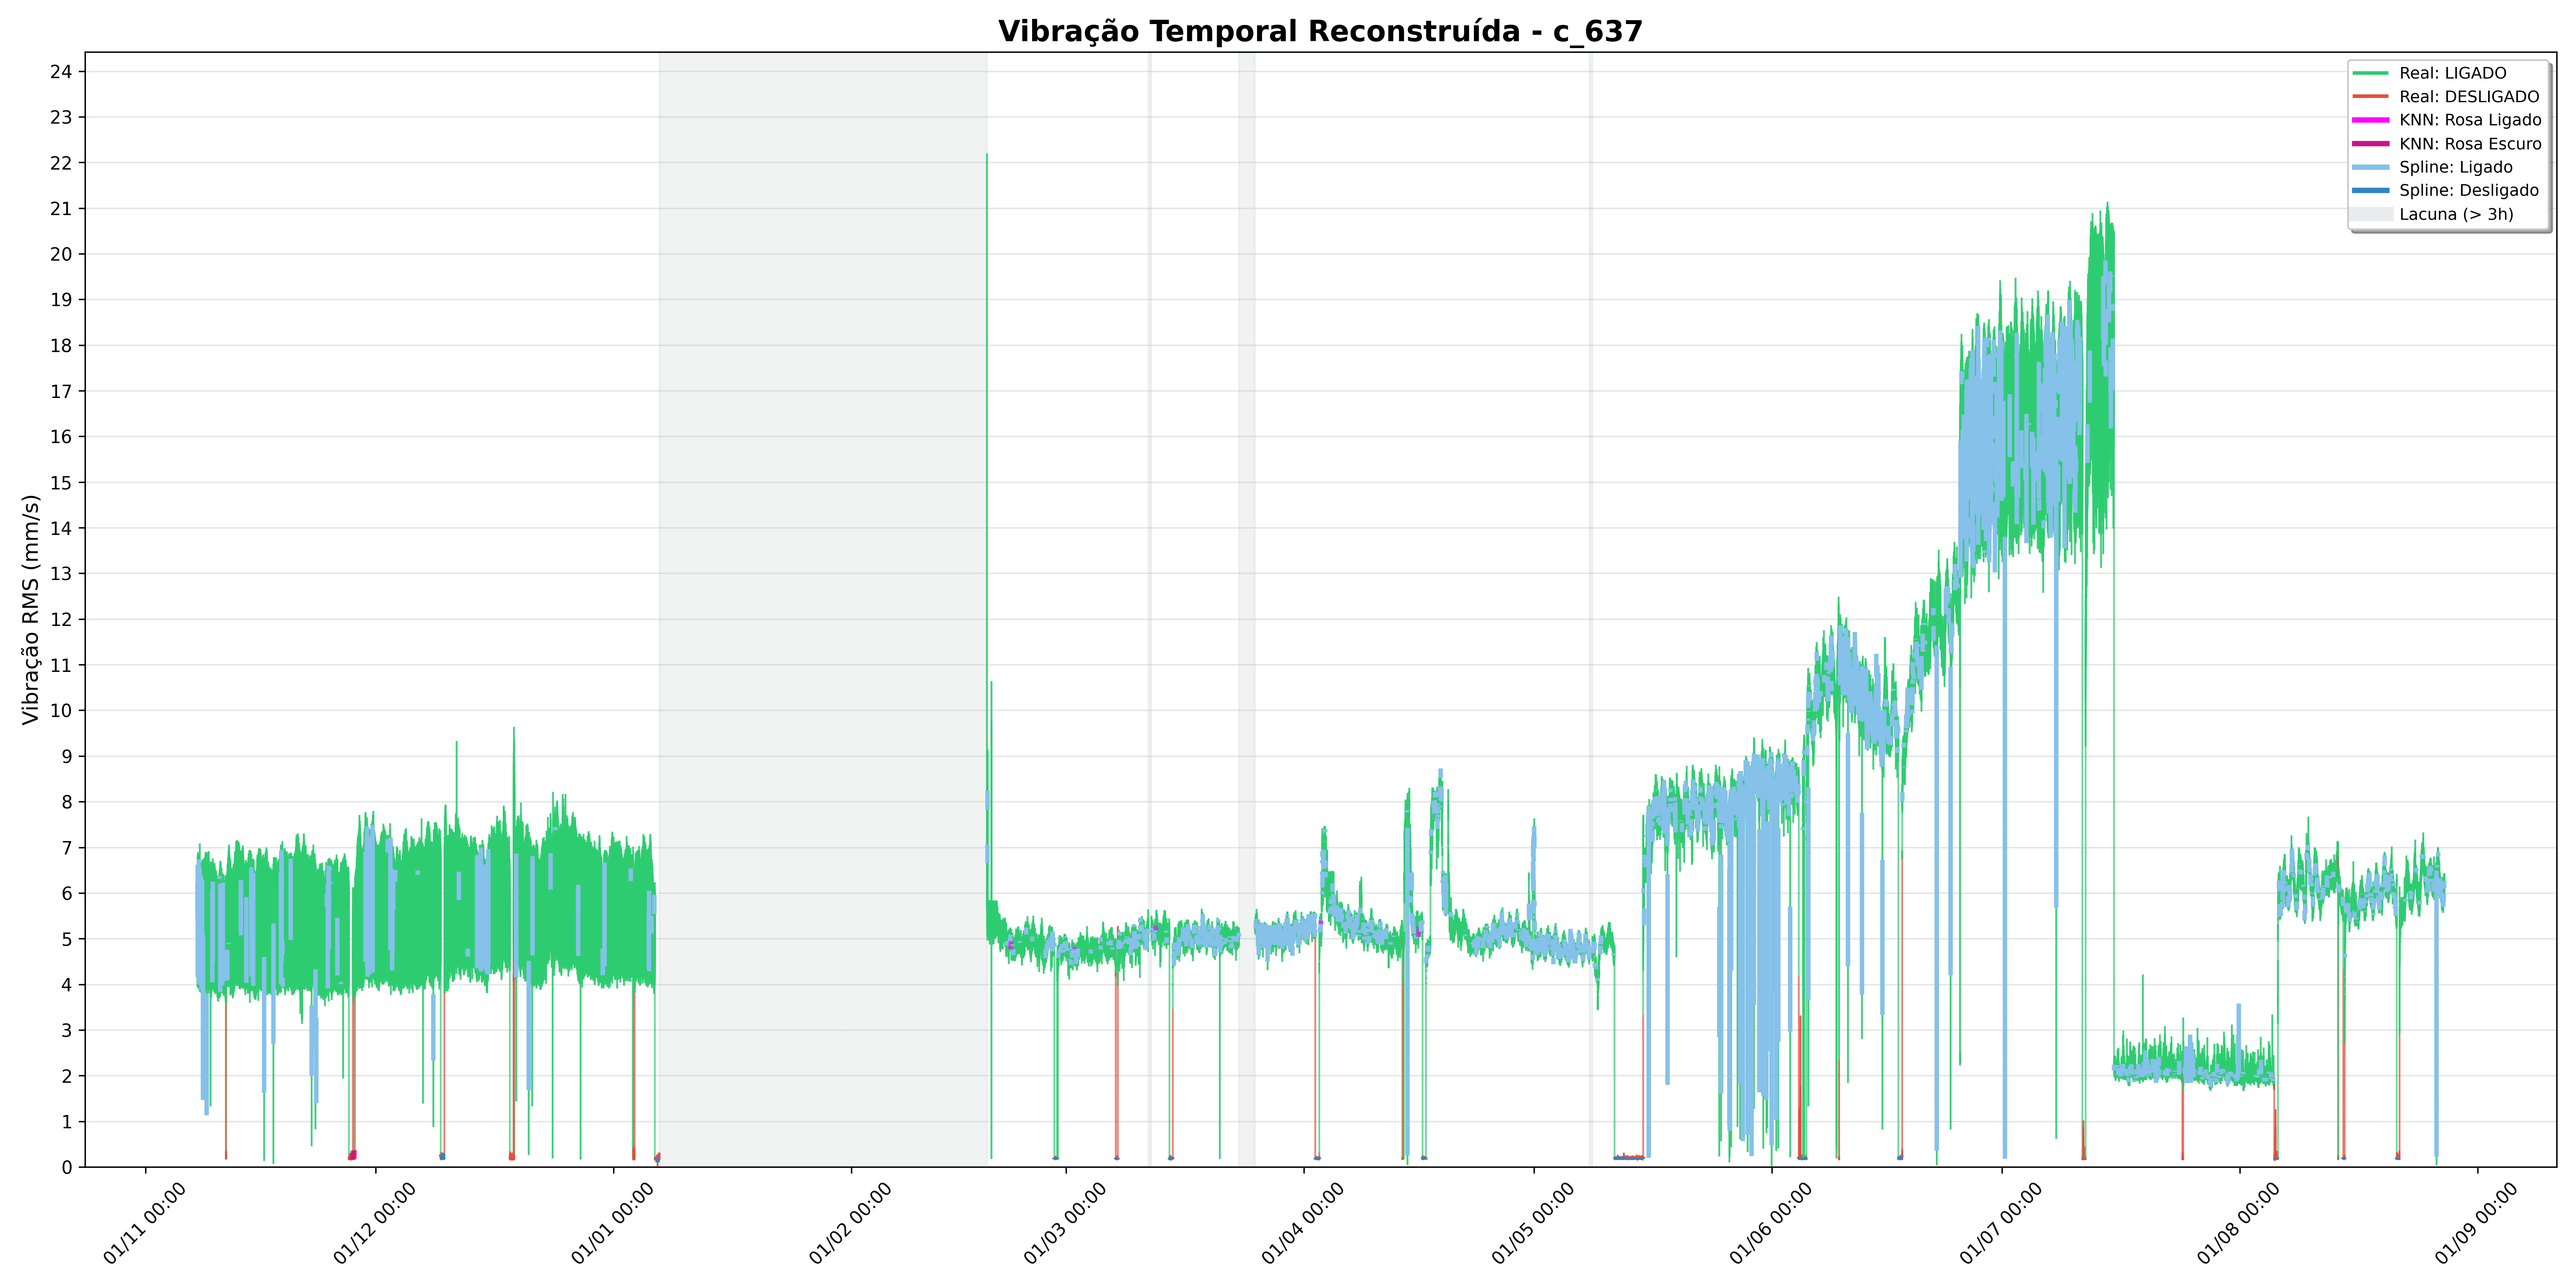
\includegraphics[width=0.85\textwidth]{results/vibracao_reconstrucao_c_637.png}
    \caption{Reconstrução temporal da vibração RMS -- $c_{637}$ (motobomba elétrica). Operação predominantemente contínua com 95,5\% do tempo em estado LIGADO.}
    \label{fig:vibracao_c_637}
\end{figure}

A Figura~\ref{fig:vibracao_c_640} exibe a reconstrução do equipamento $c_{640}$ (Motor REC), com padrão operacional similar aos demais elétricos.

\begin{figure}[H]
    \centering
    
\includegraphics[width=0.85\textwidth]{results/vibracao_reconstrucao_c_640.png}
    \caption{Reconstrução temporal da vibração RMS -- $c_{640}$ (Motor REC). 1.389.174 amostras classificadas com 94,4\% em estado LIGADO.}
    \label{fig:vibracao_c_640}
\end{figure}

A Figura~\ref{fig:vibracao_c_1518} apresenta a reconstrução do equipamento mecânico $c_{1518}$ (mancal), classificado exclusivamente por temperatura e vibração, com operação quase contínua (95,2\% LIGADO).

\begin{figure}[H]
    \centering
    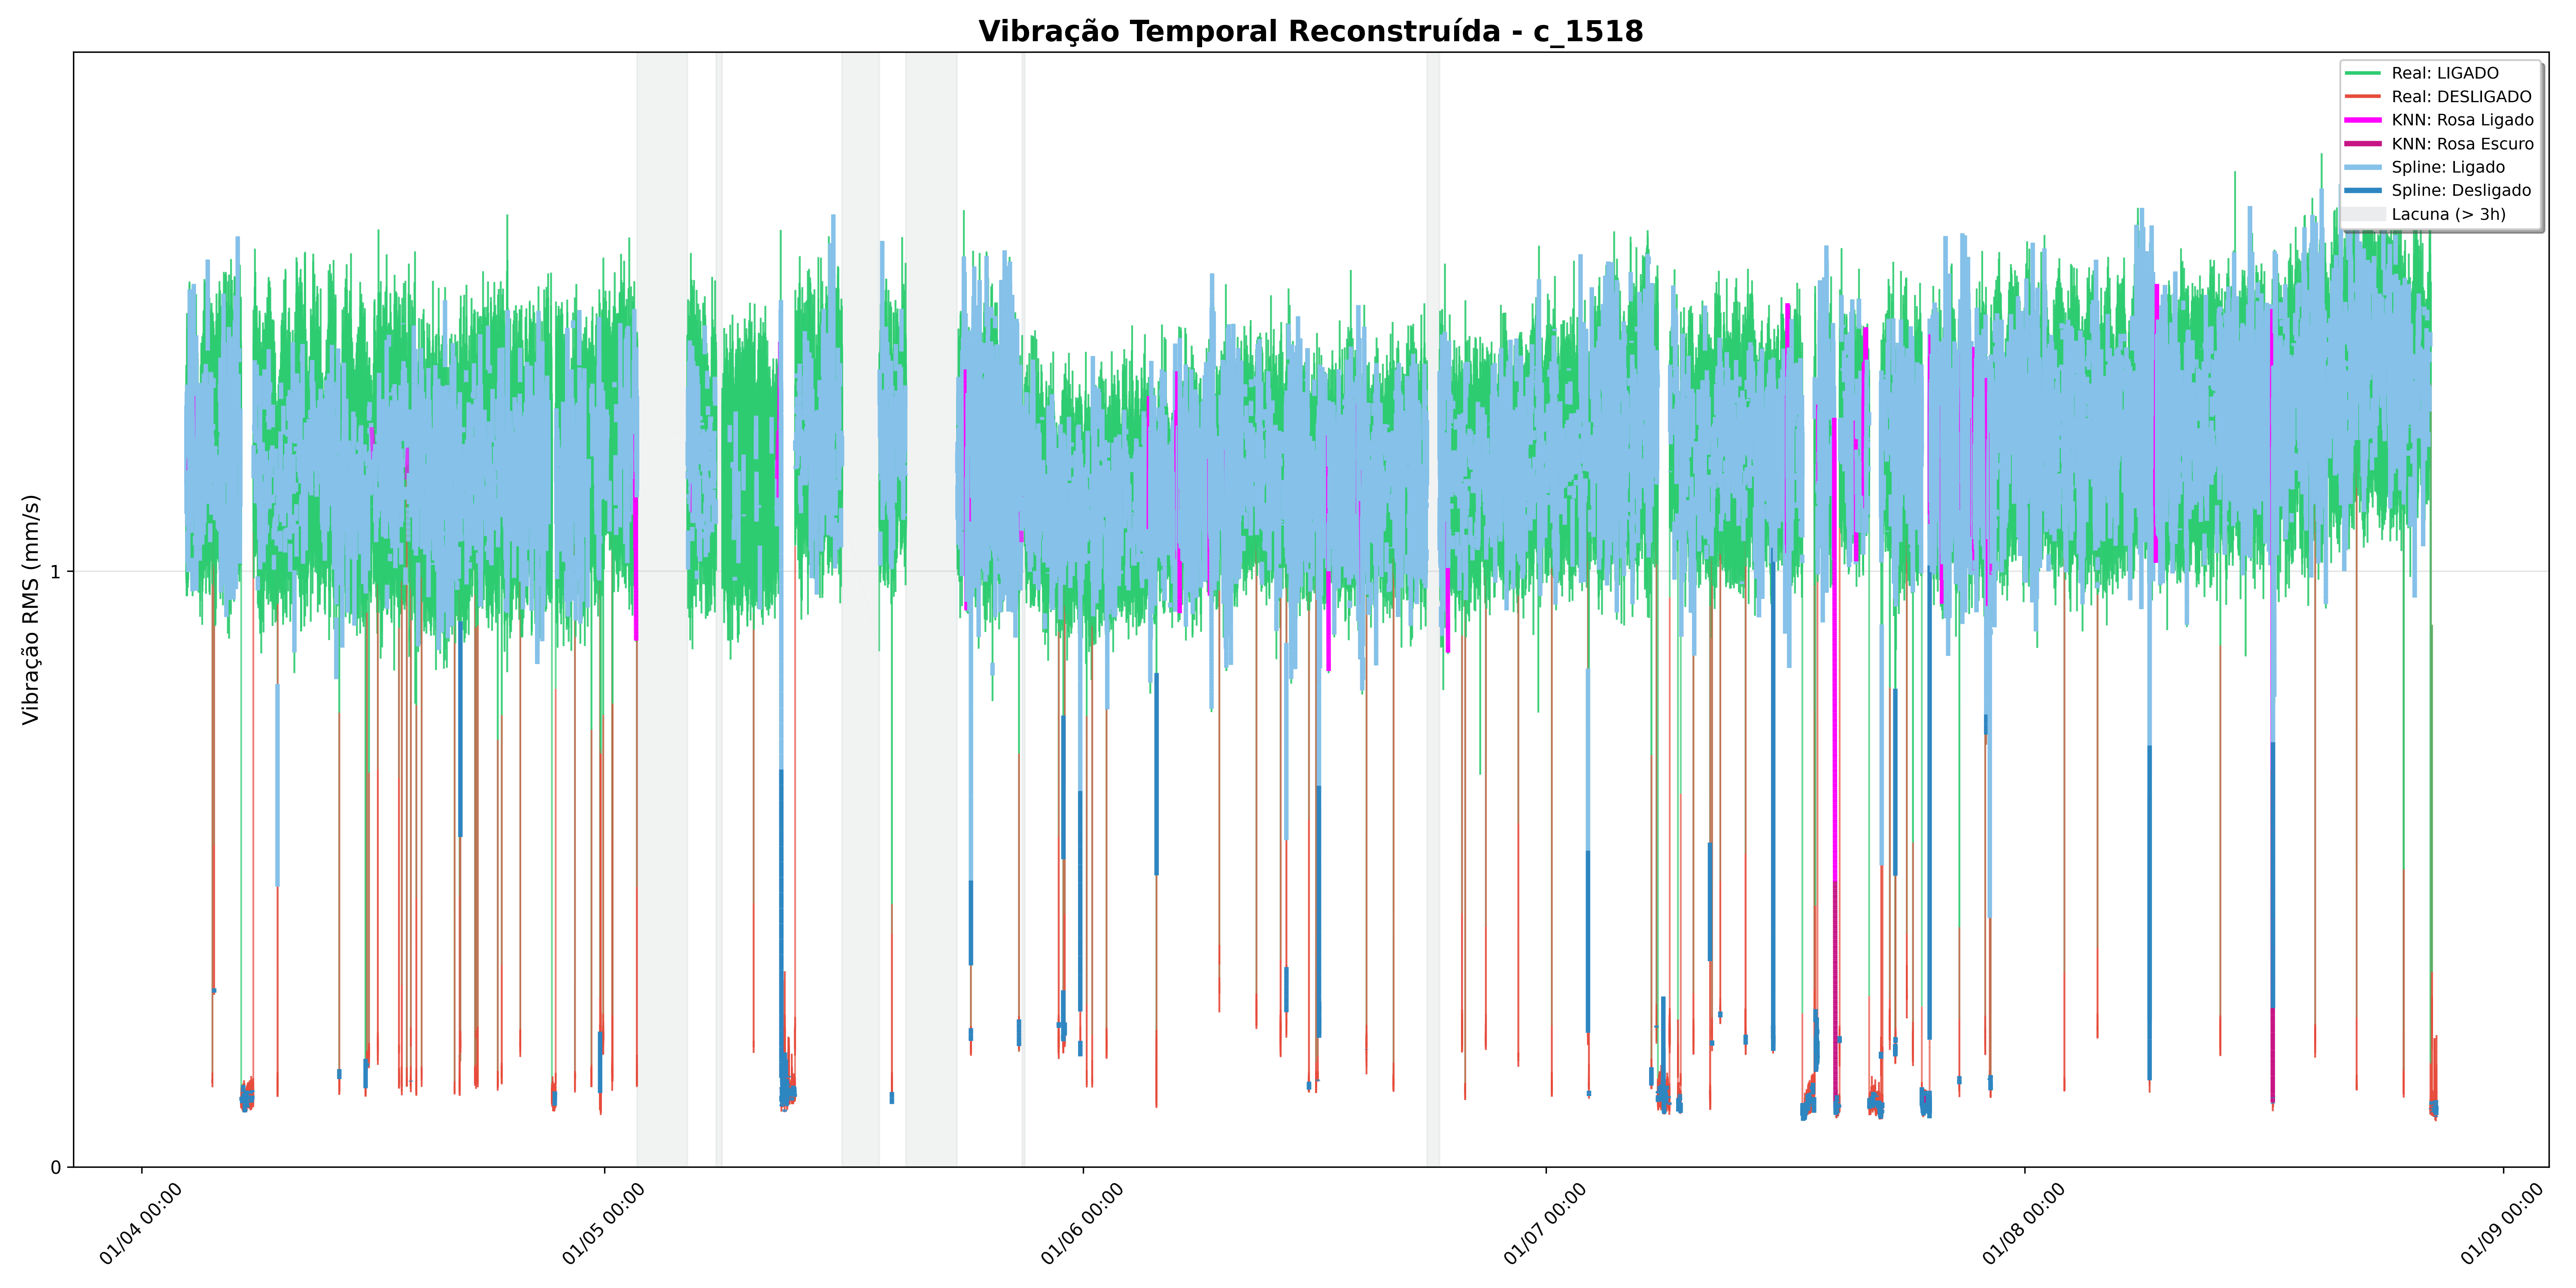
\includegraphics[width=0.85\textwidth]{results/vibracao_reconstrucao_c_1518.png}
    \caption{Reconstrução temporal da vibração RMS -- $c_{1518}$ (mancal mecânico). Classificação baseada em temperatura e vibração com 95,2\% em estado LIGADO.}
    \label{fig:vibracao_c_1518}
\end{figure}

Por fim, a Figura~\ref{fig:vibracao_c_670} mostra a reconstrução do equipamento mecânico $c_{670}$ (redutora \textit{bridle}), que apresenta a maior proporção de tempo DESLIGADO entre os mecânicos (21\%), com transições frequentes entre estados.

\begin{figure}[H]
    \centering
    
\includegraphics[width=0.85\textwidth]{results/vibracao_reconstrucao_c_670.png}
    \caption{Reconstrução temporal da vibração RMS -- $c_{670}$ (redutora \textit{bridle} mecânica). Maior proporção de DESLIGADO (21\%) entre os equipamentos mecânicos, com 1.377.884 amostras.}
    \label{fig:vibracao_c_670}
\end{figure}

\section{Aplicabilidade Prática}

O \textit{pipeline} K-Means foi validado com sucesso em cenários industriais variados. A análise histórica permitiu processar meses de dados por equipamento, gerando métricas de utilização e horímetro precisas, com relatórios automáticos e classificação sem erros, oferecendo uma base confiável para planejamento de manutenção preventiva. Para intervalos específicos de horas ou dias, o \textit{pipeline} possibilitou investigação detalhada de padrões operacionais e detecção de anomalias, com visualizações 3D de alta resolução temporal, facilitando diagnósticos rápidos. A classificação automática demonstrou robustez em qualquer intervalo com dados suficientes, garantindo LIGADO/DESLIGADO sem intervenção manual e precisão completa consistente.

A Tabela~\ref{tab:interpolacao_horas} apresenta a quantidade de dados interpolados para o equipamento $c_{637}$, discriminada por método de interpolação. No total, 157,83 horas de dados foram reconstruídas, sendo 141,74 horas via PCHIP (lacunas $\leq$ 30 minutos) e 16,09 horas via KNN multivariado (lacunas entre 30 minutos e 3 horas). Esses valores representam apenas 2,3\% do total de dados processados, demonstrando que a grande maioria do sinal é composta por dados originais do sensor.

\begin{table}[H]
    \centering
    \caption{Horas interpoladas por método -- Equipamento $c_{637}$}
    \label{tab:interpolacao_horas}
    \begin{tabular}{|l|r|r|r|}
        \hline
        Método                & Pontos    & Horas    & Qualidade \\
        \hline
        PCHIP ($\leq$ 30 min) & 25.514    & 141,74   & 0,95      \\
        KNN (30 min -- 3h)    & 2.896     & 16,09    & 0,75      \\
        \hline
        Total interpolado     & 28.410    & 157,83   & ---       \\
        Dados originais       & 1.214.583 & 6.747,68 & 1,00      \\
        \hline
    \end{tabular}
\end{table}

Os benefícios operacionais incluem precisão total na tomada de decisão, automação completa do processo, escalabilidade para milhões de registros, interpretabilidade dos resultados por meio de visualizações compreensíveis e robustez frente a dados não utilizados no treinamento.

Algumas limitações técnicas foram identificadas. Durante a fase de treinamento, períodos com lacunas superiores a três horas são descartados automaticamente para preservar a qualidade dos centróides, e dados insuficientes podem invalidar a criação do modelo. O modelo é específico para cada equipamento e a classificação é binária, focada apenas em estados LIGADO e DESLIGADO, sem detecção de anomalias operacionais. Na prática, o \textit{pipeline} requer um conjunto inicial de dados para treinamento (mínimo recomendado de 30 dias), opera \textit{offline}, depende de infraestrutura de dados adequada e concentra-se na classificação de estados, sem predição de falhas.

A síntese dos resultados mostra que o \textit{pipeline} K-Means é uma solução robusta e eficaz para a classificação automática de estados operacionais em equipamentos industriais. Ele permite processar grandes volumes de dados de forma eficiente, mantém desempenho consistente com dados novos, fornece resultados interpretáveis e opera de forma totalmente automatizada. O \textit{pipeline} se mostrou escalável e confiável em diferentes equipamentos industriais, desde motobombas até motores e componentes mecânicos como mancais e redutoras, oferecendo simplicidade, robustez e resultados consistentes para aplicações industriais práticas.